\documentclass[xcolor=table]{beamer}
\usetheme[progressbar=frametitle]{metropolis}
\usepackage{appendixnumberbeamer}

\usepackage[absolute,overlay]{textpos}
\usepackage{booktabs}
\usepackage{pgf, tikz}
\usepackage{pdfcomment}
\usepackage{pgfplots}
\usepackage{hyperref}
\usepackage[utf8]{inputenc}
\usepackage{xspace}
\usepackage{color}
\newcommand{\themename}{\textbf{\textsc{metropolis}}\xspace}
\newcommand\FontImportant{\fontsize{15}{20}\selectfont}
\newcommand\FontMoyenImportant{\fontsize{14}{17}\selectfont}
\newcommand\FontPetit{\fontsize{8}{6}\selectfont}
\title{Simulation de formes réalistes de développement résidentiel, de l'échelle du bâtiment à celle de l'ensemble d'une région urbaine}
\author{Maxime Colomb}
\subtitle{\textit{Sous la direction de M. Brasebin, J. Perret \& C. Tannier}
	\\Soutenance de thèse}

\titlegraphic{
\includegraphics[height=1.1cm]{Images/logoIGN.png}\hfill
\includegraphics[height=1.1cm]{Images/logoThema.jpg}}

\makeatletter
\newcommand\addsectiontotoc[1]{%
  \addtocontents{toc}{%
    \protect\beamer@sectionintoc{\the\c@section}{#1}{\the\c@page}{\the\c@part}%
                                {\the\beamer@tocsectionnumber}}
}
\makeatother

\makeatletter
\newcommand{\miniscule}{\@setfontsize\miniscule{4}{5}}% \tiny: 5/6
\makeatother

\setbeamerfont*{section in head/foot}{size=\miniscule}
\setbeamercolor{section in head/foot}{parent=palette primary}

\addtobeamertemplate{frametitle}{}{%
  \begin{textblock*}{5cm}(11cm,0.1cm)
    \insertsectionnavigation{4cm}
  \end{textblock*}
}
\begin{document}

\maketitle
\section{Introduction}
\begin{frame}{Contexte : le phénomène d'étalement urbain}
	\begin{block}{}
		\begin{itemize}
			\item Répond aux souhaits d'un grand nombre de ménages
			\item Multiples effets négatifs
			\item Objectif de régulation des pouvoirs publics
		\end{itemize}
		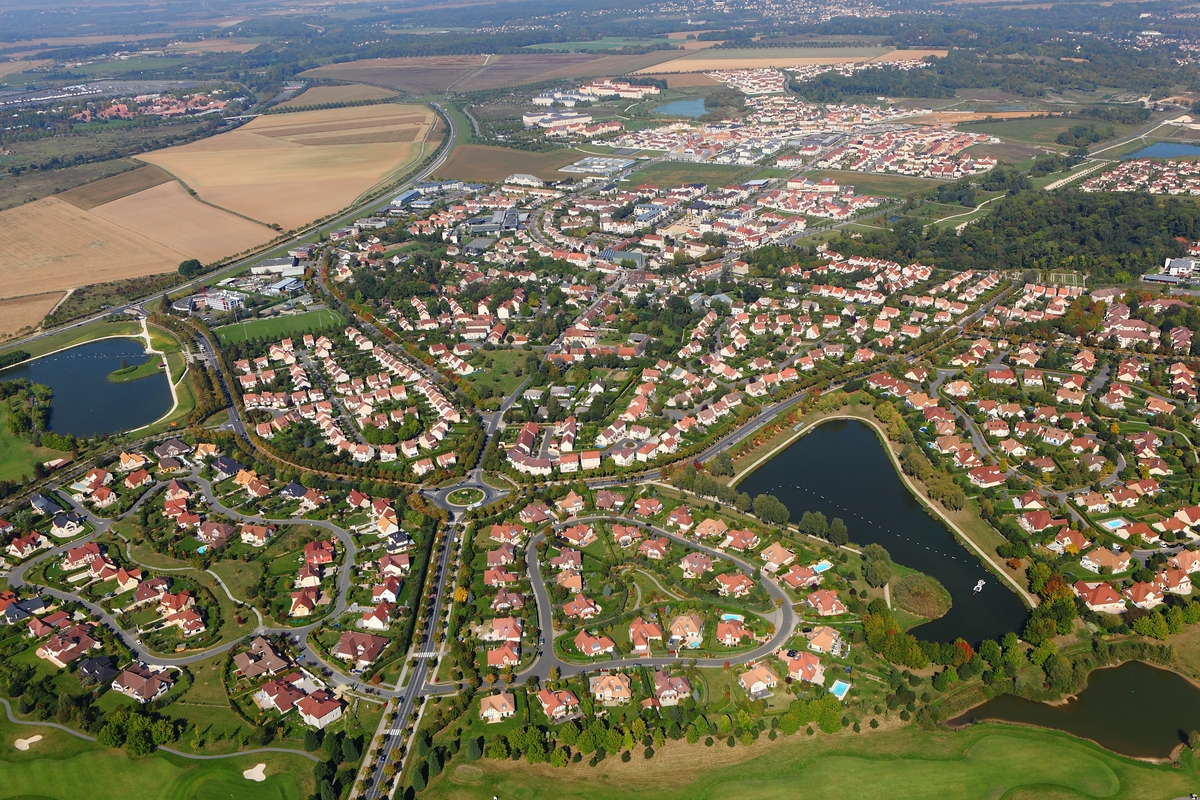
\includegraphics[height=2.5cm]{Images/consome.jpg}
		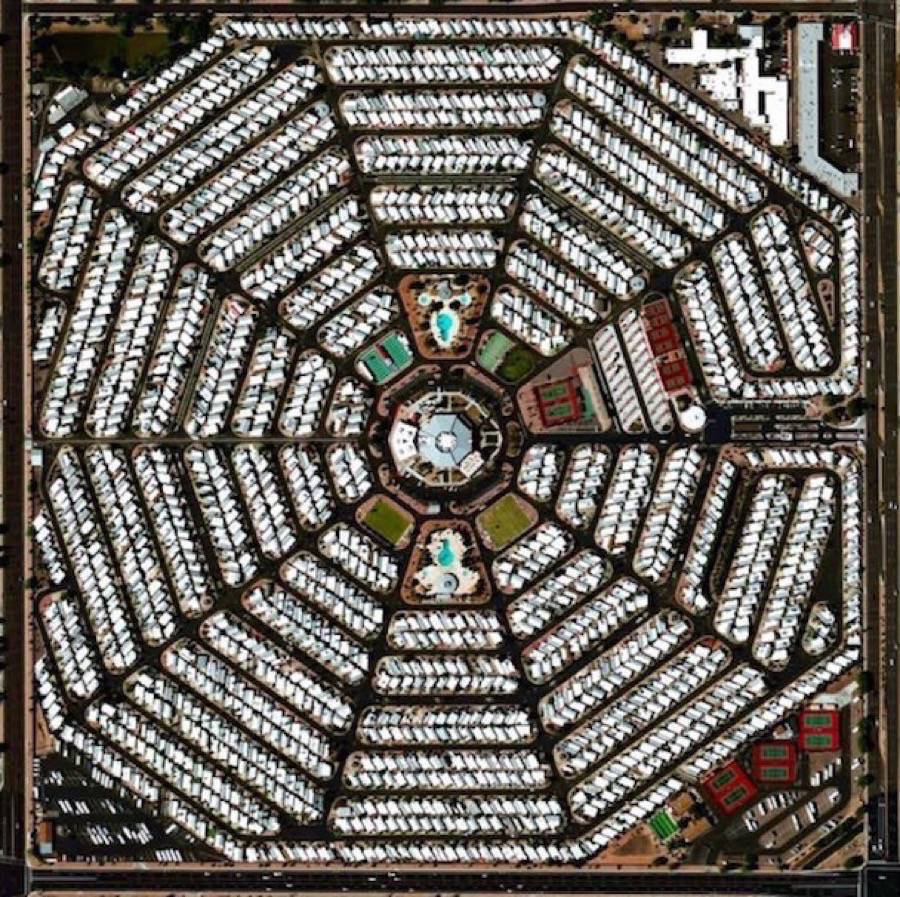
\includegraphics[height=2.5cm]{Images/sto.jpeg}
		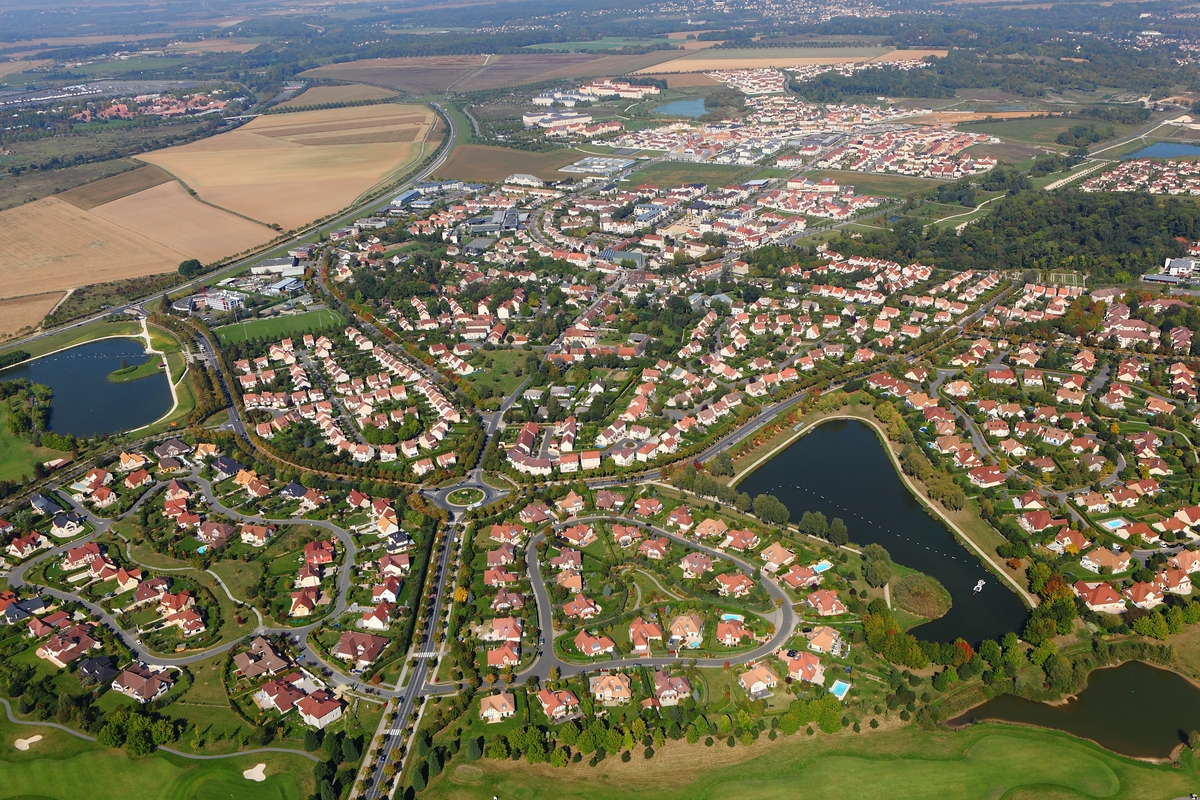
\includegraphics[height=2.5cm]{Images/consome.jpg}
	\end{block}
	\begin{block}{}
	\uncover<2>{Dynamiques résidentielles prépondérantes (Joly 03, Wiel 13)}
		%Le logement étant le principal levier de ce développement, nous nous concentrons sur le développement résidentiel 
	\end{block}
\end{frame}

\begin{frame}{Divers documents d'aménagement réglementant l'extension résidentielle} 
	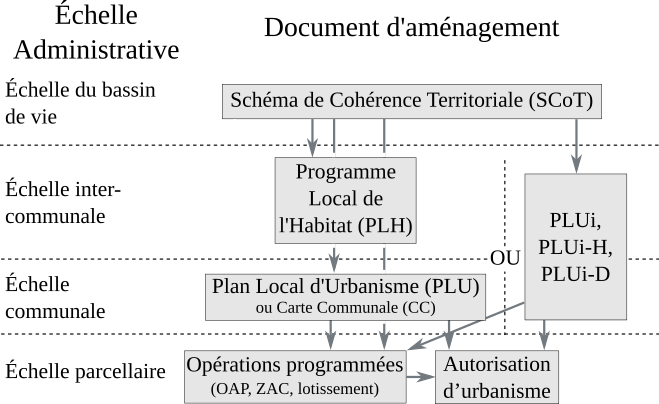
\includegraphics[width=11cm]{Images/planification-globale-Prez.png}
\end{frame}

\begin{frame}{Différents types de contraintes réglementaires} 
	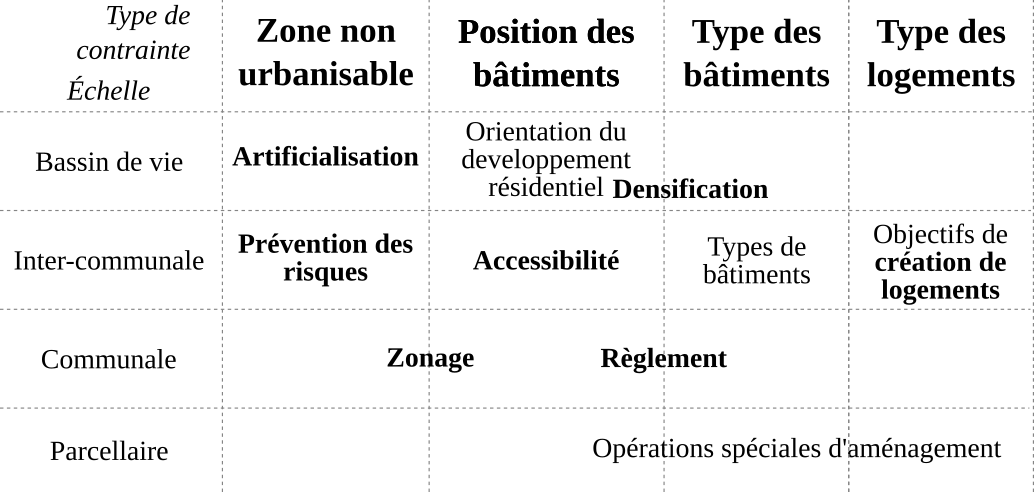
\includegraphics[width=11cm]{Images/synthese-doc.png}
\end{frame}

\begin{frame}{Enjeux : compatibilité/conformité des documents d'urbanisme}
	\begin{itemize}
		\item Différents \textbf{rédacteurs}
		\item Objectifs divers
		\item Différentes \textbf{échelles} d'application
		\item Effets incertains 
		\item Combinaison potentiellement \textbf{contradictoire}
	\end{itemize}
	\uncover<2->{	
		\begin{block}{}
		\textbf{Modéliser l'articulation de ces contraintes pour tester leurs combinaison}
%			Représenter l'articulation entre les différents documents de plannificaiton et d'urbanisme grâce à un modèle de simulation afin de tester la combinaison des différentes règles et contraintes d'aménagements
%			\textbf{Tester} les effets combinés des documents d'urbanisme sur le développement résidentiel afin de \textbf{représenter} leurs \textbf{articulation} grâce à la \textbf{modélisation} %et d'expliciter leurs \textbf{}
		\end{block}
	}
\end{frame}

\begin{frame}{Le contenu de la modélisation}
	\begin{itemize}
		\item<1-> Simuler le développement résidentiel à différents niveaux d'échelles et selon plusieurs contraintes
		\item<2-> Exprimer divers critères d'évaluation de la plannification~:
		\begin{itemize}	
			\item<3-> La création de logements
			\item<4-> La densité de logements par hectare
			\item<5-> L'accessibilité (aux transports en communs, ...)
		\end{itemize}
		\vspace{0.66cm}
		\item<6-> Représentation des états intermédiaires non nécessaire
		\item<7-> Pas de reproduction des phénomènes anterieurs
		\vspace{0.66cm}
		\item<8-> Solutions libres et open-source pour une recherche \textbf{vérifiable} et \textbf{reproductible}
		\item<9> Utilisation de modèles préexistants
	\end{itemize}
\end{frame}

\begin{frame}<1-2>[label=EA]
\frametitle{État de l'art des solutions existantes}
\begin{block}{}
		\alert<2>{$\star$ Objectif~: Modèle prospectif d'aide à la décision}
\end{block}
\begin{block}{}
		\alert<3>{$\star$ Modélisation de phénomènes géographiques}
\end{block}
\begin{block}{}
		\alert<4>{$\star$ Approches intégrées}
\end{block}
\begin{block}{}
		\alert<5>{$\star$ Modèles génératifs}
\end{block}
\end{frame}

\begin{frame}{Les outils d'aide à la décision pour l'aménagement à visée prospective}
	\begin{block}{}
		\textbf{Objectifs}\\
		Modélise \textbf{un ou plusieurs phénomènes} réels\\
		Simule l'état du système étudié face à ce(s) phénomène(s)\\
	%	Simulations réapplicables et systématisables\\
	\end{block}
	\uncover<2->{	
		\begin{block}{}
			\textbf{Utilisations}\\
			Permettre de comparer plusieurs \textbf{scénarios}\\	
			Représenter des futurs potentiels, recherchés, redoutés\\
			Utilisation en tant qu'\textbf{outil} pour l'\textbf{aide} à la conception de documents %et non pour une rédaction \textit{automatisée} - Possibilitées plutôt que prédictions
		\end{block}
	}
	\uncover<3>{De nombreux outils \textit{spatialement explicites} à visée prospective existent}
\end{frame}


\begin{frame}{État de l'art des outils d'aide à la décision dans l'aménagement à visée prospective}
	\only<1>{Les modèles d'\textbf{aide à la décision multi-critères} (ref) permettent de~: %TODO ref
	\begin{itemize}
		\item Prendre en compte de nombreux paramètres pondérés pour dégager une décision
		\item Pondérer les différents systèmes intéressants pour le développement résidentiel
	\end{itemize}
	Problèmes des modèles d'\textbf{aide à la décision multi-critères}~:
	\begin{itemize}
		\item Solutions pré-déterminées
		\item Un phénomène plutôt qu'une interaction complexe entre différents systèmes
	\end{itemize}
	}
	\only<2>{
	Les modèles d'\textbf{étude du marché immobilier} (UrbanSimul (), ...) premettent de %TODO ref
	\begin{itemize}
		\item Analyser le marché de l'immobilier, la pression foncière
		\item Propose des prédictions sur l'état du marché et sur les futures urbanisations
	\end{itemize}
	Inconvénients~: 
	\begin{itemize}
			\item Peu adaptés pour représenter la compléxité des mécanismes multi-échelles d'un développement résidentiel 
			\item Résultats dépendant principalement du marché et non des objectifs de la planification
%			\item Très contextualisé
	\end{itemize}}
	\only<3>{Ces outils sont appliqués à la résolution d'\textbf{un} problème défini et sont \textbf{peu interopérable}}
\end{frame}

\againframe<3>{EA}

\begin{frame}{État de l'art des modèles simulant le développement résidentiel}
	\only<1>{Modélisation de phénomènes complexes grâce à des objets géométriques \textit{simplifiés}\\} %TODO redire
	\only<2>{Les \textbf{automates cellulaires} (Yeh 2015, Mustafa 2018) sont utilisés pour~:
		\begin{itemize}
			\item fournir une représentation synthétique et simplifiée de l'espace grâce à un carroyage
			\item simuler des changements d'états dynamiques pour chacune des cellules en fonction d'équations 
		\end{itemize}
	Inconvénients~: 
		\begin{itemize}
			\item ne pas traiter des formes géographiques complexes (parcelles, bâtiments)
		\end{itemize}
	}
	\only<3>{
	Les \textbf{modèles Multi-Agents} (Artznete 10, ...) permettent de~:
	\begin{itemize}
		\item représenter un système en reproduisant les comportements d'agents et leurs interactions ;
		\item faire émerger des configurations particulières
	\end{itemize}
	Inconvénients~:
		\begin{itemize}
			\item très forte dynamiques
			\item modélisation de notre problème trop compliquée %(définition des agents, des interactions et des contraintes)
		\end{itemize}
	}
	\only<4>{Les modèles simplifiés ne sont pas assez descriptifs pour représenter le développement résidentiel à un niveau très local}
\end{frame}

\againframe<4>{EA}

\begin{frame}{État de l'art des modèles intégrés simulant le développement résidentiel}
		Les approches intégrées, telles que les LUTI (Land-Use and Transportation Interaction), permettent de~:
		\begin{itemize}
			\item simuler les interactions entre différents modèles (occupation du sol, mobilités, systèmes économiques ...) 
			\item articuler différents systèmes modélisés 
			\item avoir une approche \textit{prospective} %TODO redire
		\end{itemize}
		Inconvénients~:
		\begin{itemize}
			\item mise en œuvre conséquente 
			\item modélisation des mobilités non nécessaire à notre problème
		\end{itemize}
		\uncover<2>{Approches intéressantes du \textbf{couplage} de \textbf{modules} agissant à \textbf{différentes échelles}}
	
\end{frame}

\againframe<5>{EA}

\begin{frame}{État de l'art des modèles génératifs de développements résidentiels}
	\only<1>{Génération d'îlots urbains}
	\only<2>{Génération de parcelles}
	\only<3>{Génération de bâtiments}
	%À une échelle très locale, d'autre dynamiques et d'autre types de modèles
	%	(trouver des références sur l'étude des parcelles cf. rapport JT)
	\begin{itemize}
		\item<1-2> processus géo-historiques \only<1>{GeOpenSim (Perret 2010)} \only<2>{(Perret 2015)} 
		\item<2-> génération procédurale \only<2>{(Vanegas 2012)} \only<3>{(BIM)} 
		\item<2-> génération paramétrique \only<2>{(Yazýcý 2016)} \only<3>{(Coors 2009)}
		\item<3> optimisation sous contrainte (Brasebin 2014)
	\end{itemize}
\end{frame}

\begin{frame}{Problématique}
	\only<1>{Il n'existe pas de modèles permettant de simuler un développement résidentiel multi-échelles, multi-contraint et suffisamment descriptif pour s'adapter aux contraintes locales.}
	\only<2>{Comment \textbf{simuler} le \textbf{développement résidentiel} d'une région urbaine à un niveau \textbf{très détaillé}, afin d'identifier et d'explorer les effets combinés des différents types de \textbf{documents de planification et d'urbanisme} ?}
\end{frame}

\begin{frame}{Objectif de la thèse}
%	\uncover<2->{\begin{block}{}
%			Comportement particulier
	%		\begin{itemize}
	%			\footnotesize
				%\item Sans calibration provenant des développements résidentiels passés pour pouvoir se concentrer sur l'effet des documents d'urbanisme 
%				\item Sans dynamique temporelles pour exprimer le potentiel de développement résidentiel à un instant précis
%			\end{itemize}
%	\end{block}}
	\begin{block}{}
		Développer un nouvel outil d'aide à la décision dans l'aménagement, couplant différentes approches, appelé \textbf{ArtiScales}
	\end{block}
\end{frame}




%\section[Plan]{Plan de la présentation}




\begin{frame}{Plan de la présentation}
	\begin{itemize}
		\item Fonctionnement d'\textbf{ArtiScales}
		\item \textbf{Modules} d'ArtiScales
		\item \textbf{Analyse et validation} des modules d'ArtiScales
		\item \textbf{Expérimentation} d'ArtiScales
	\end{itemize}
\end{frame}




\section{ArtiScales}

\begin{frame}{ArtiScales : Rappel des objectifs}
		\begin{block}{}
		Création d'un modèle de développement résidentiel~:
		\begin{itemize}
			\footnotesize
			\item réaliste %(respectant les règlements et les contraintes physiques et fonctionnelles)
			\item multi-échelles %(d'une région urbaine à la parcelle)
			\item soumis à diverses contraintes %(reprsentant diffrents mécanismes et objectifs)
			\item ouvert %(vérifiable et reproductible) %\textit{Préciser les objectifs (back/forecasting)} ? ou avant? 
		\end{itemize}
	\end{block}
\end{frame}

\begin{frame}{ArtiScales : Fonctionnement}
	\centering
	\only<1>{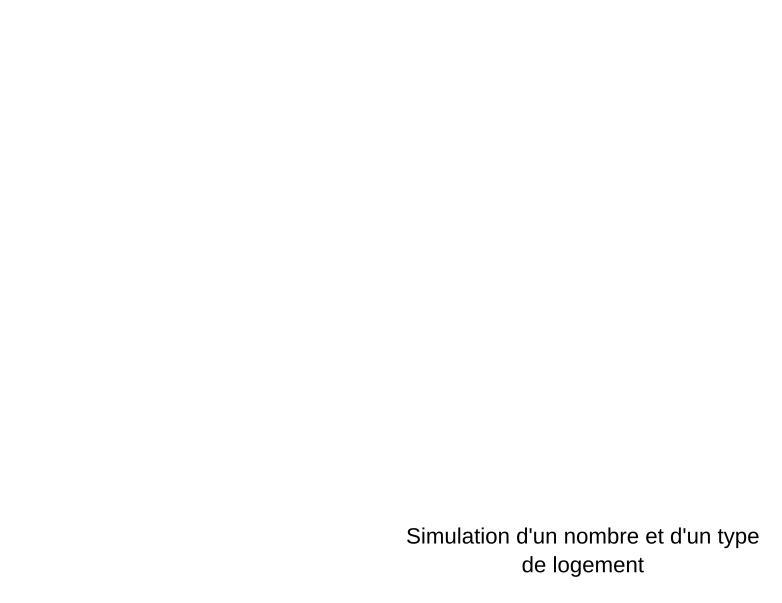
\includegraphics[width=11.5cm]{Images/schemGenPrez0.png}}
	\only<2>{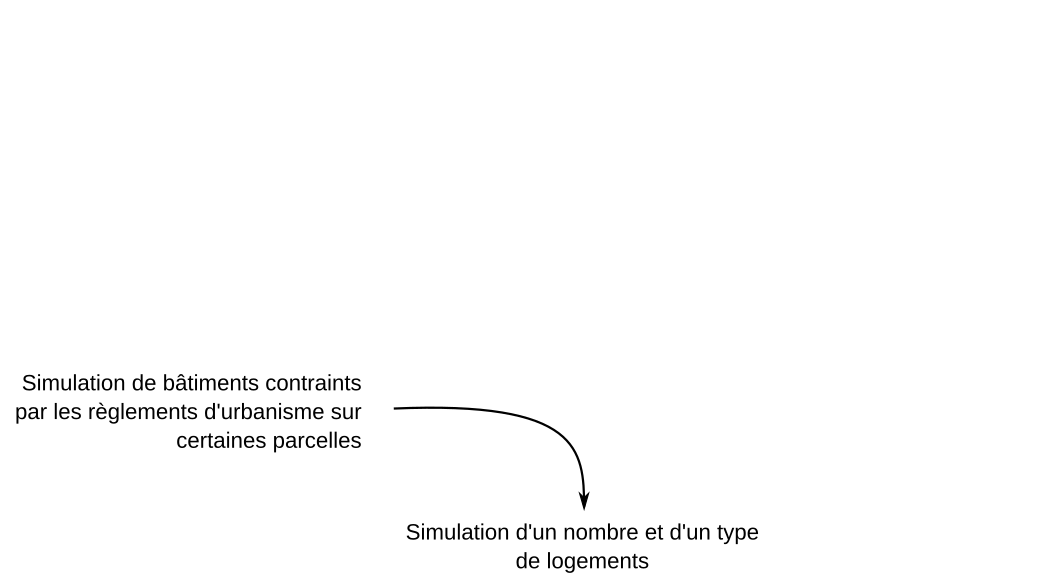
\includegraphics[width=11.5cm]{Images/schemGenPrez1.png}}
	\only<3>{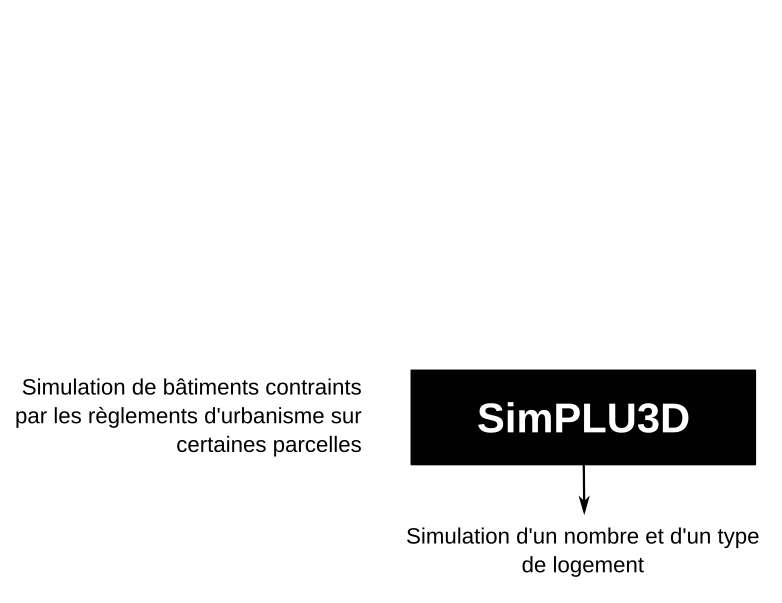
\includegraphics[width=11.5cm]{Images/schemGenPrez2.png}}
	\only<4>{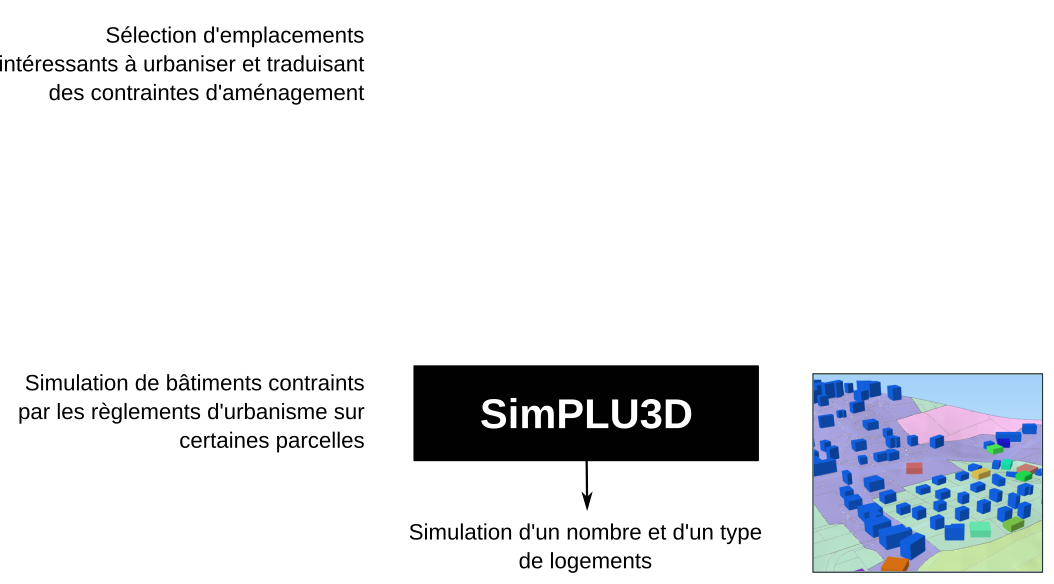
\includegraphics[width=11.5cm]{Images/schemGenPrez3.png}}
	\only<5>{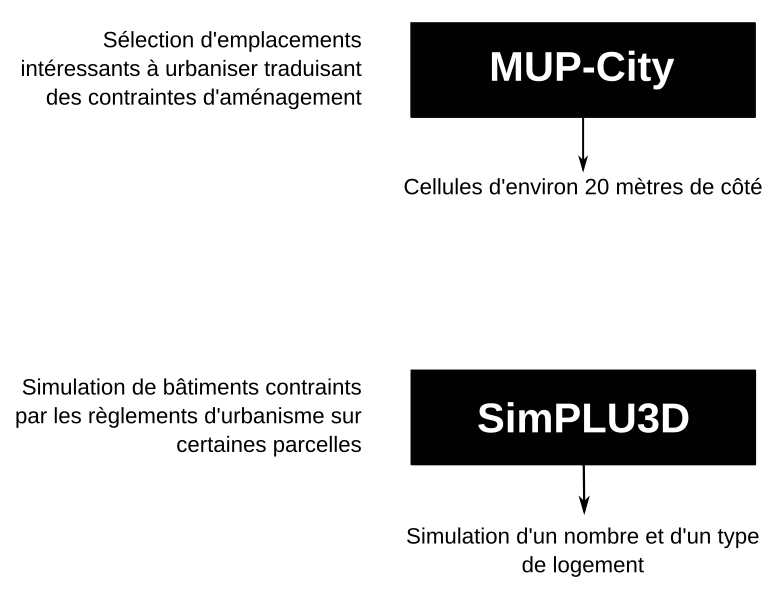
\includegraphics[width=11.5cm]{Images/schemGenPrez4.png}}
	\only<6>{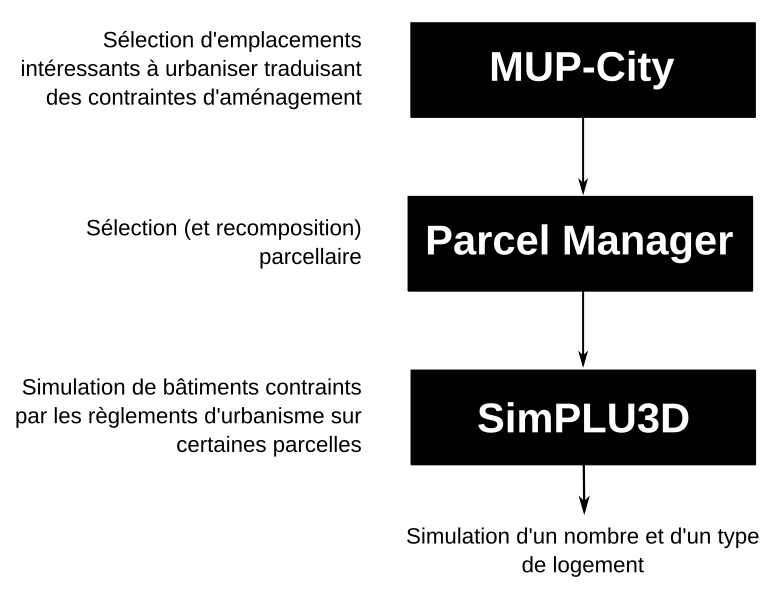
\includegraphics[width=11.5cm]{Images/schemGenPrez5.png}}
	\only<7>{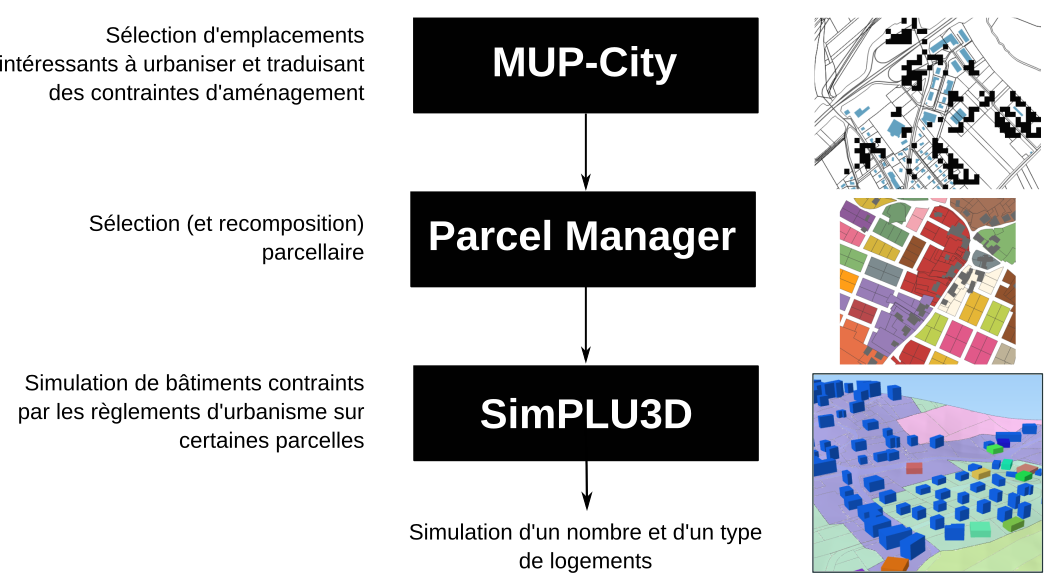
\includegraphics[width=11.5cm]{Images/schemGenPrez6.png}}
\end{frame}


\section[MUP-City]{MUP-City et l'indentification d'emplacements pour le développement résidentiel}


\begin{frame}{MUP-City : principes et objectifs}
	\centering{
\includegraphics[width=3cm]{Images/mup.png}}
	\\
	\begin{itemize}
		\item Propose une \textbf{organisation spatiale locale} de développement résidentiel pour une \textbf{région urbaine}
		\begin{itemize}
			\item<2-> organisation fractale
			\item<3-> accessibilité à diverses aménités %TODO ne plus utiliser ce mot 
		\end{itemize}
		\item<4> Représente différentes \textbf{orientations d'aménagement} grâce à de multiples paramètres.
	\end{itemize}
	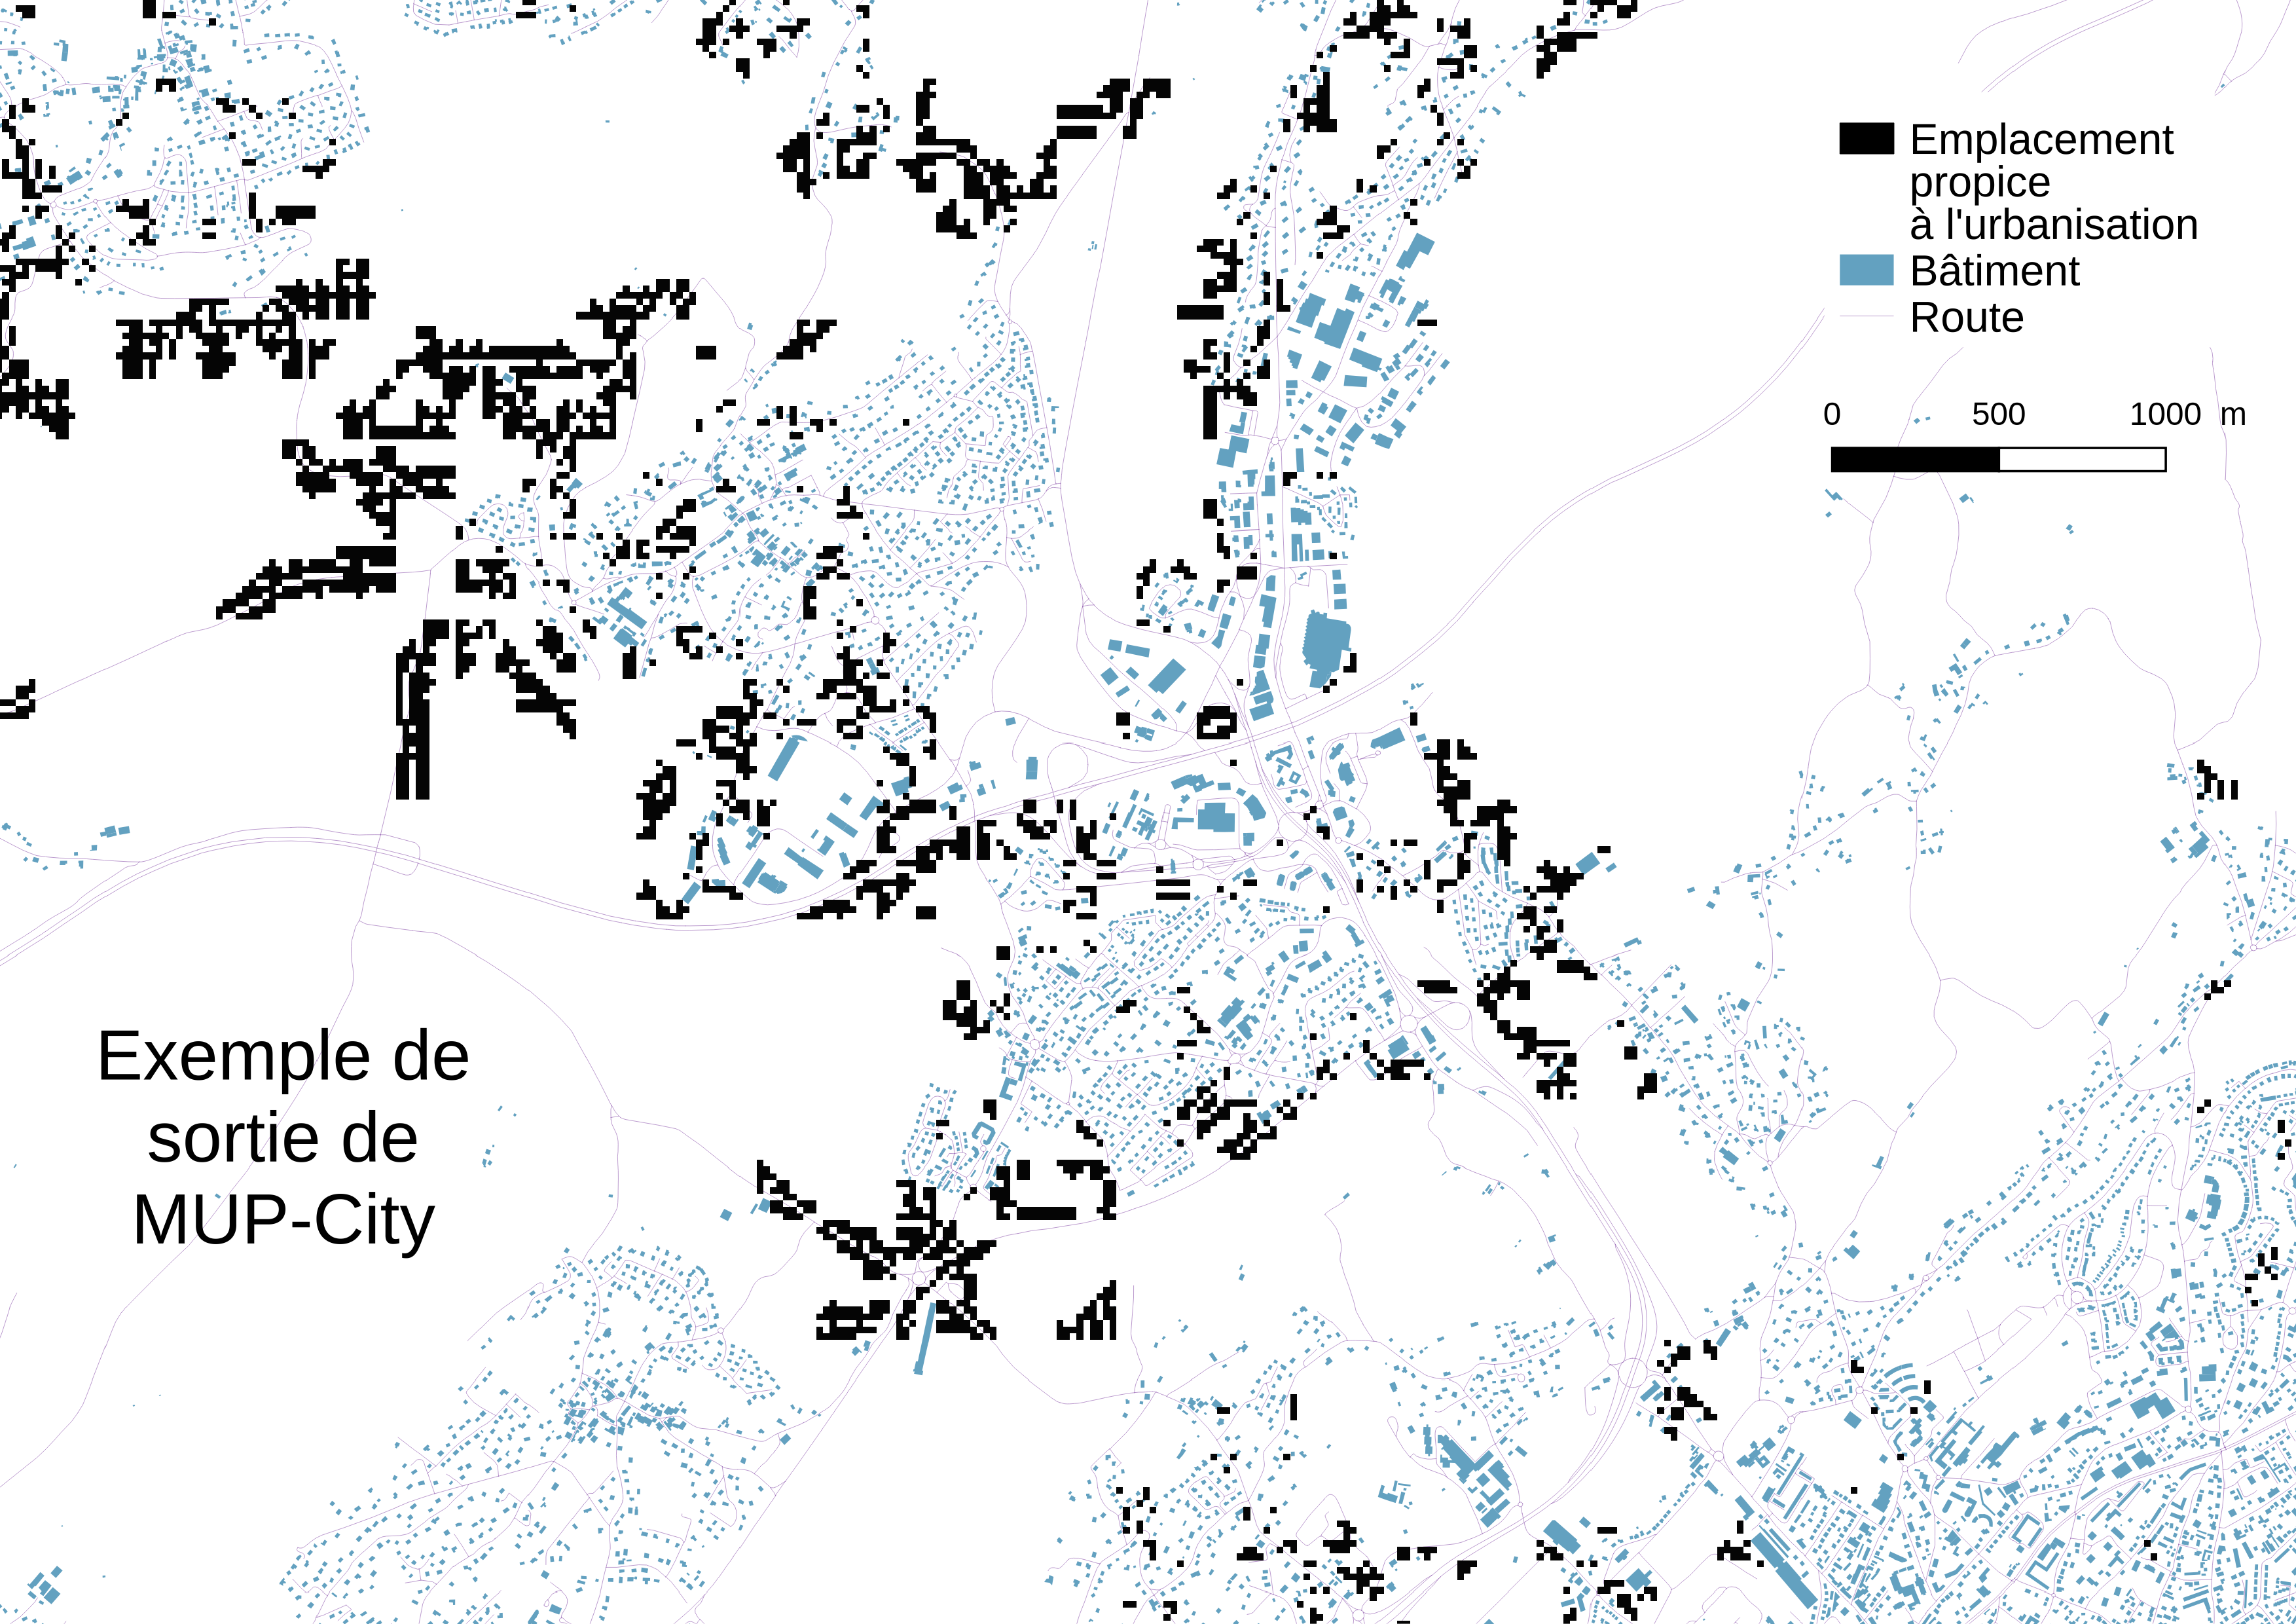
\includegraphics[width=6.5cm]{Images/ex-sorties-mup.png}
\end{frame}

\begin{frame}{MUP-City: fonctionnement}
	\begin{block}{}\centering{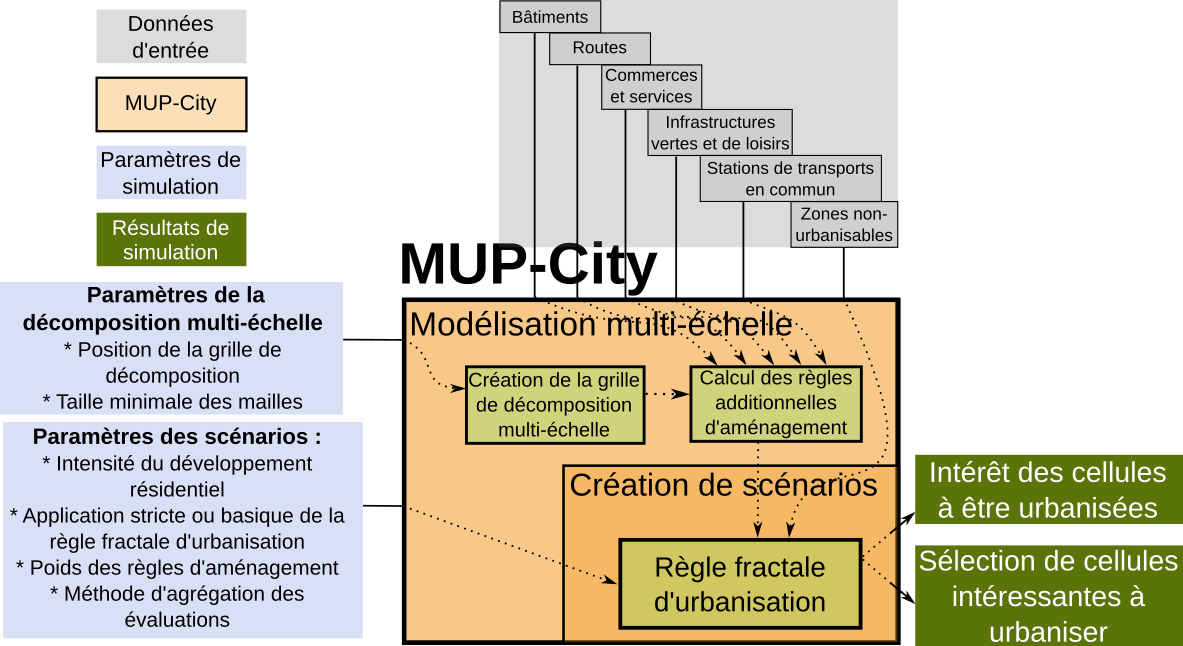
\includegraphics[width=11cm]{Images/schema-mup-city-prez.png}}\end{block}
\end{frame}


\section[Parcel Manager]{Parcel Manager pour la gestion du tissus parcellaire}

\begin{frame}{Présentation du modèle}
 	\centering
 \only<1>{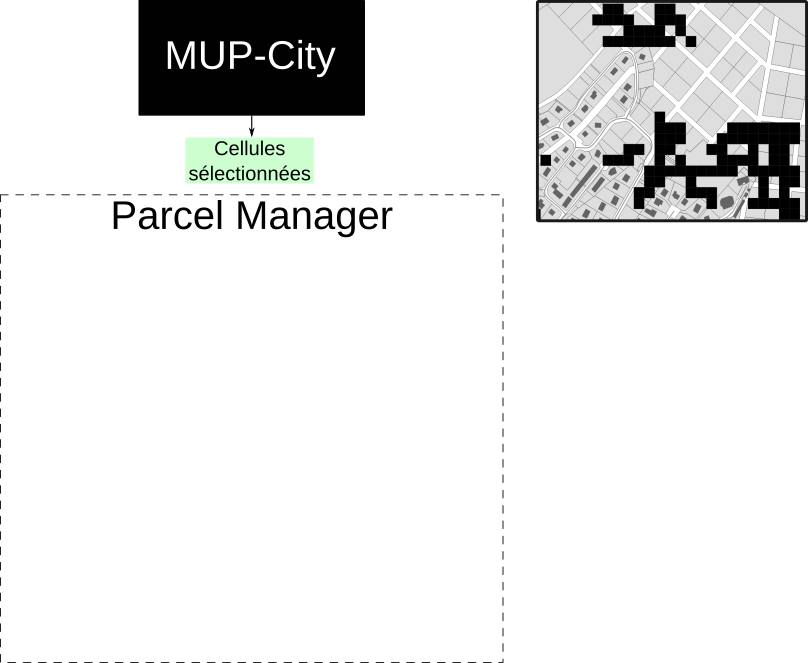
\includegraphics[width=10cm]{Images/schemGenParcelManager-prez0.png}}
 \only<2>{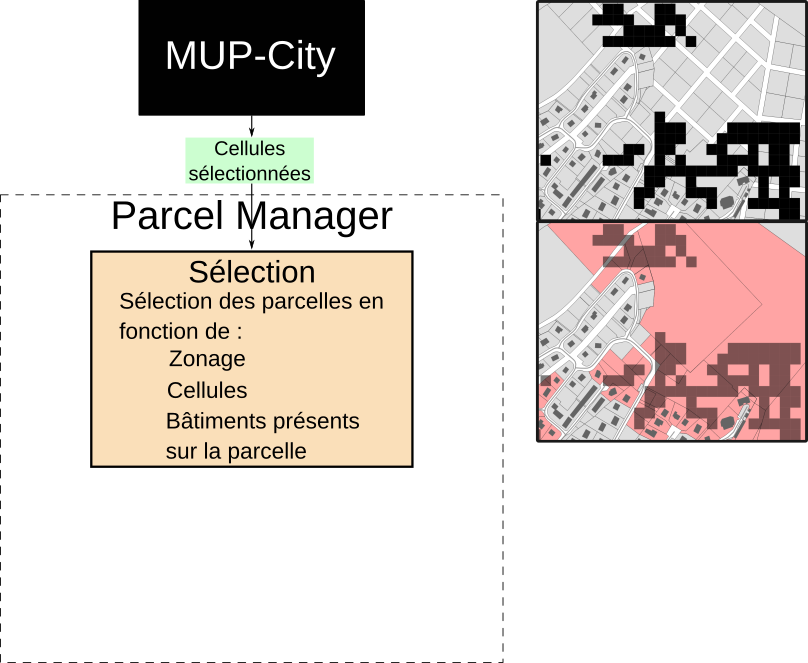
\includegraphics[width=10cm]{Images/schemGenParcelManager-prez1.png}}
 \only<3>{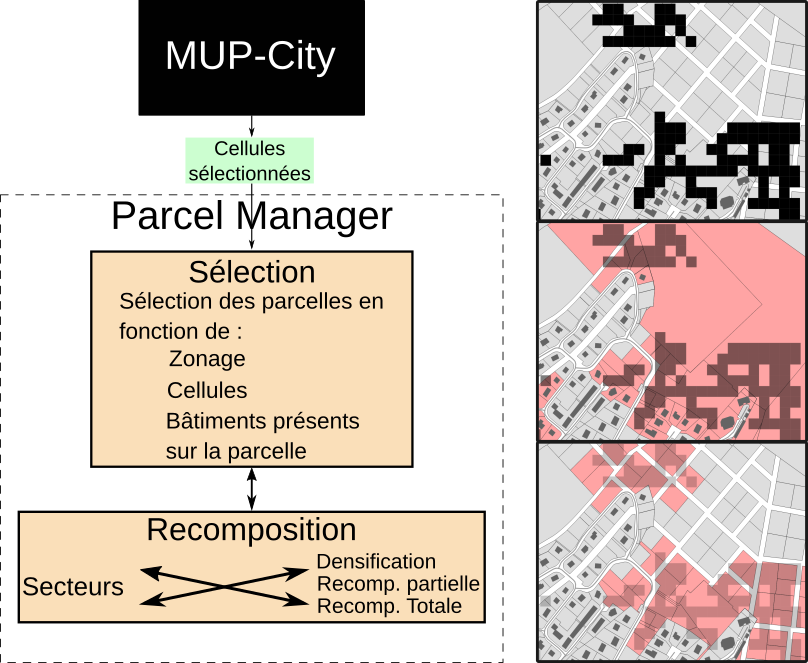
\includegraphics[width=10cm]{Images/schemGenParcelManager-prez2.png}}
\end{frame}

\begin{frame}{Algorithme de découpage parcellaire}
	\only<1>{{\footnotesize Adapté de Vannegas, 2012}
	\\
	\centering{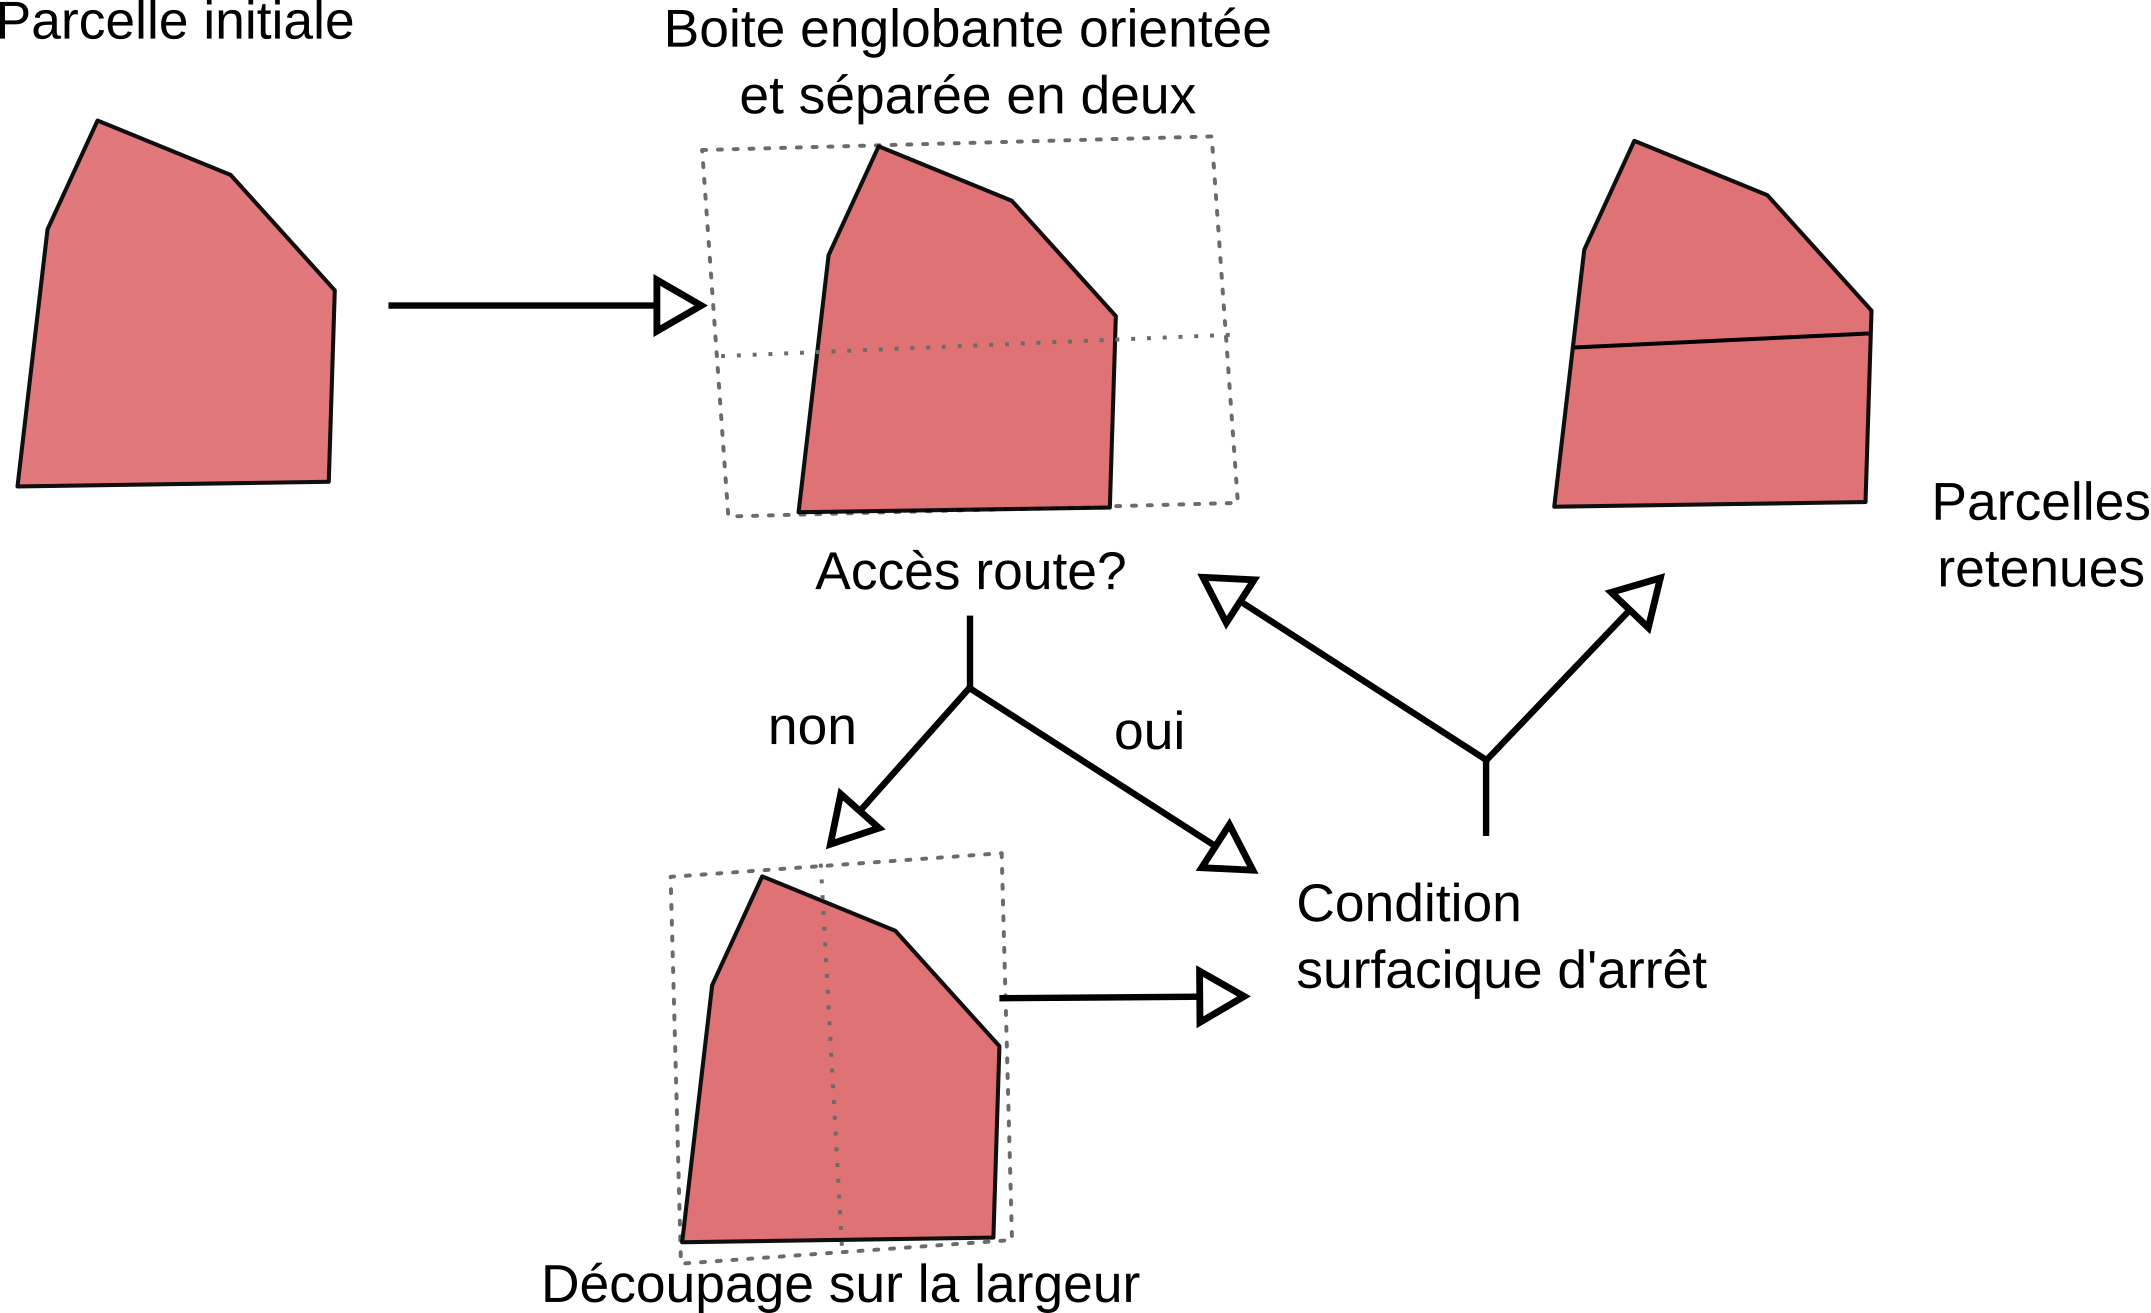
\includegraphics[width=9cm]{Images/decompositionParcelle-prez.png}}}
	\only<2>{\centering{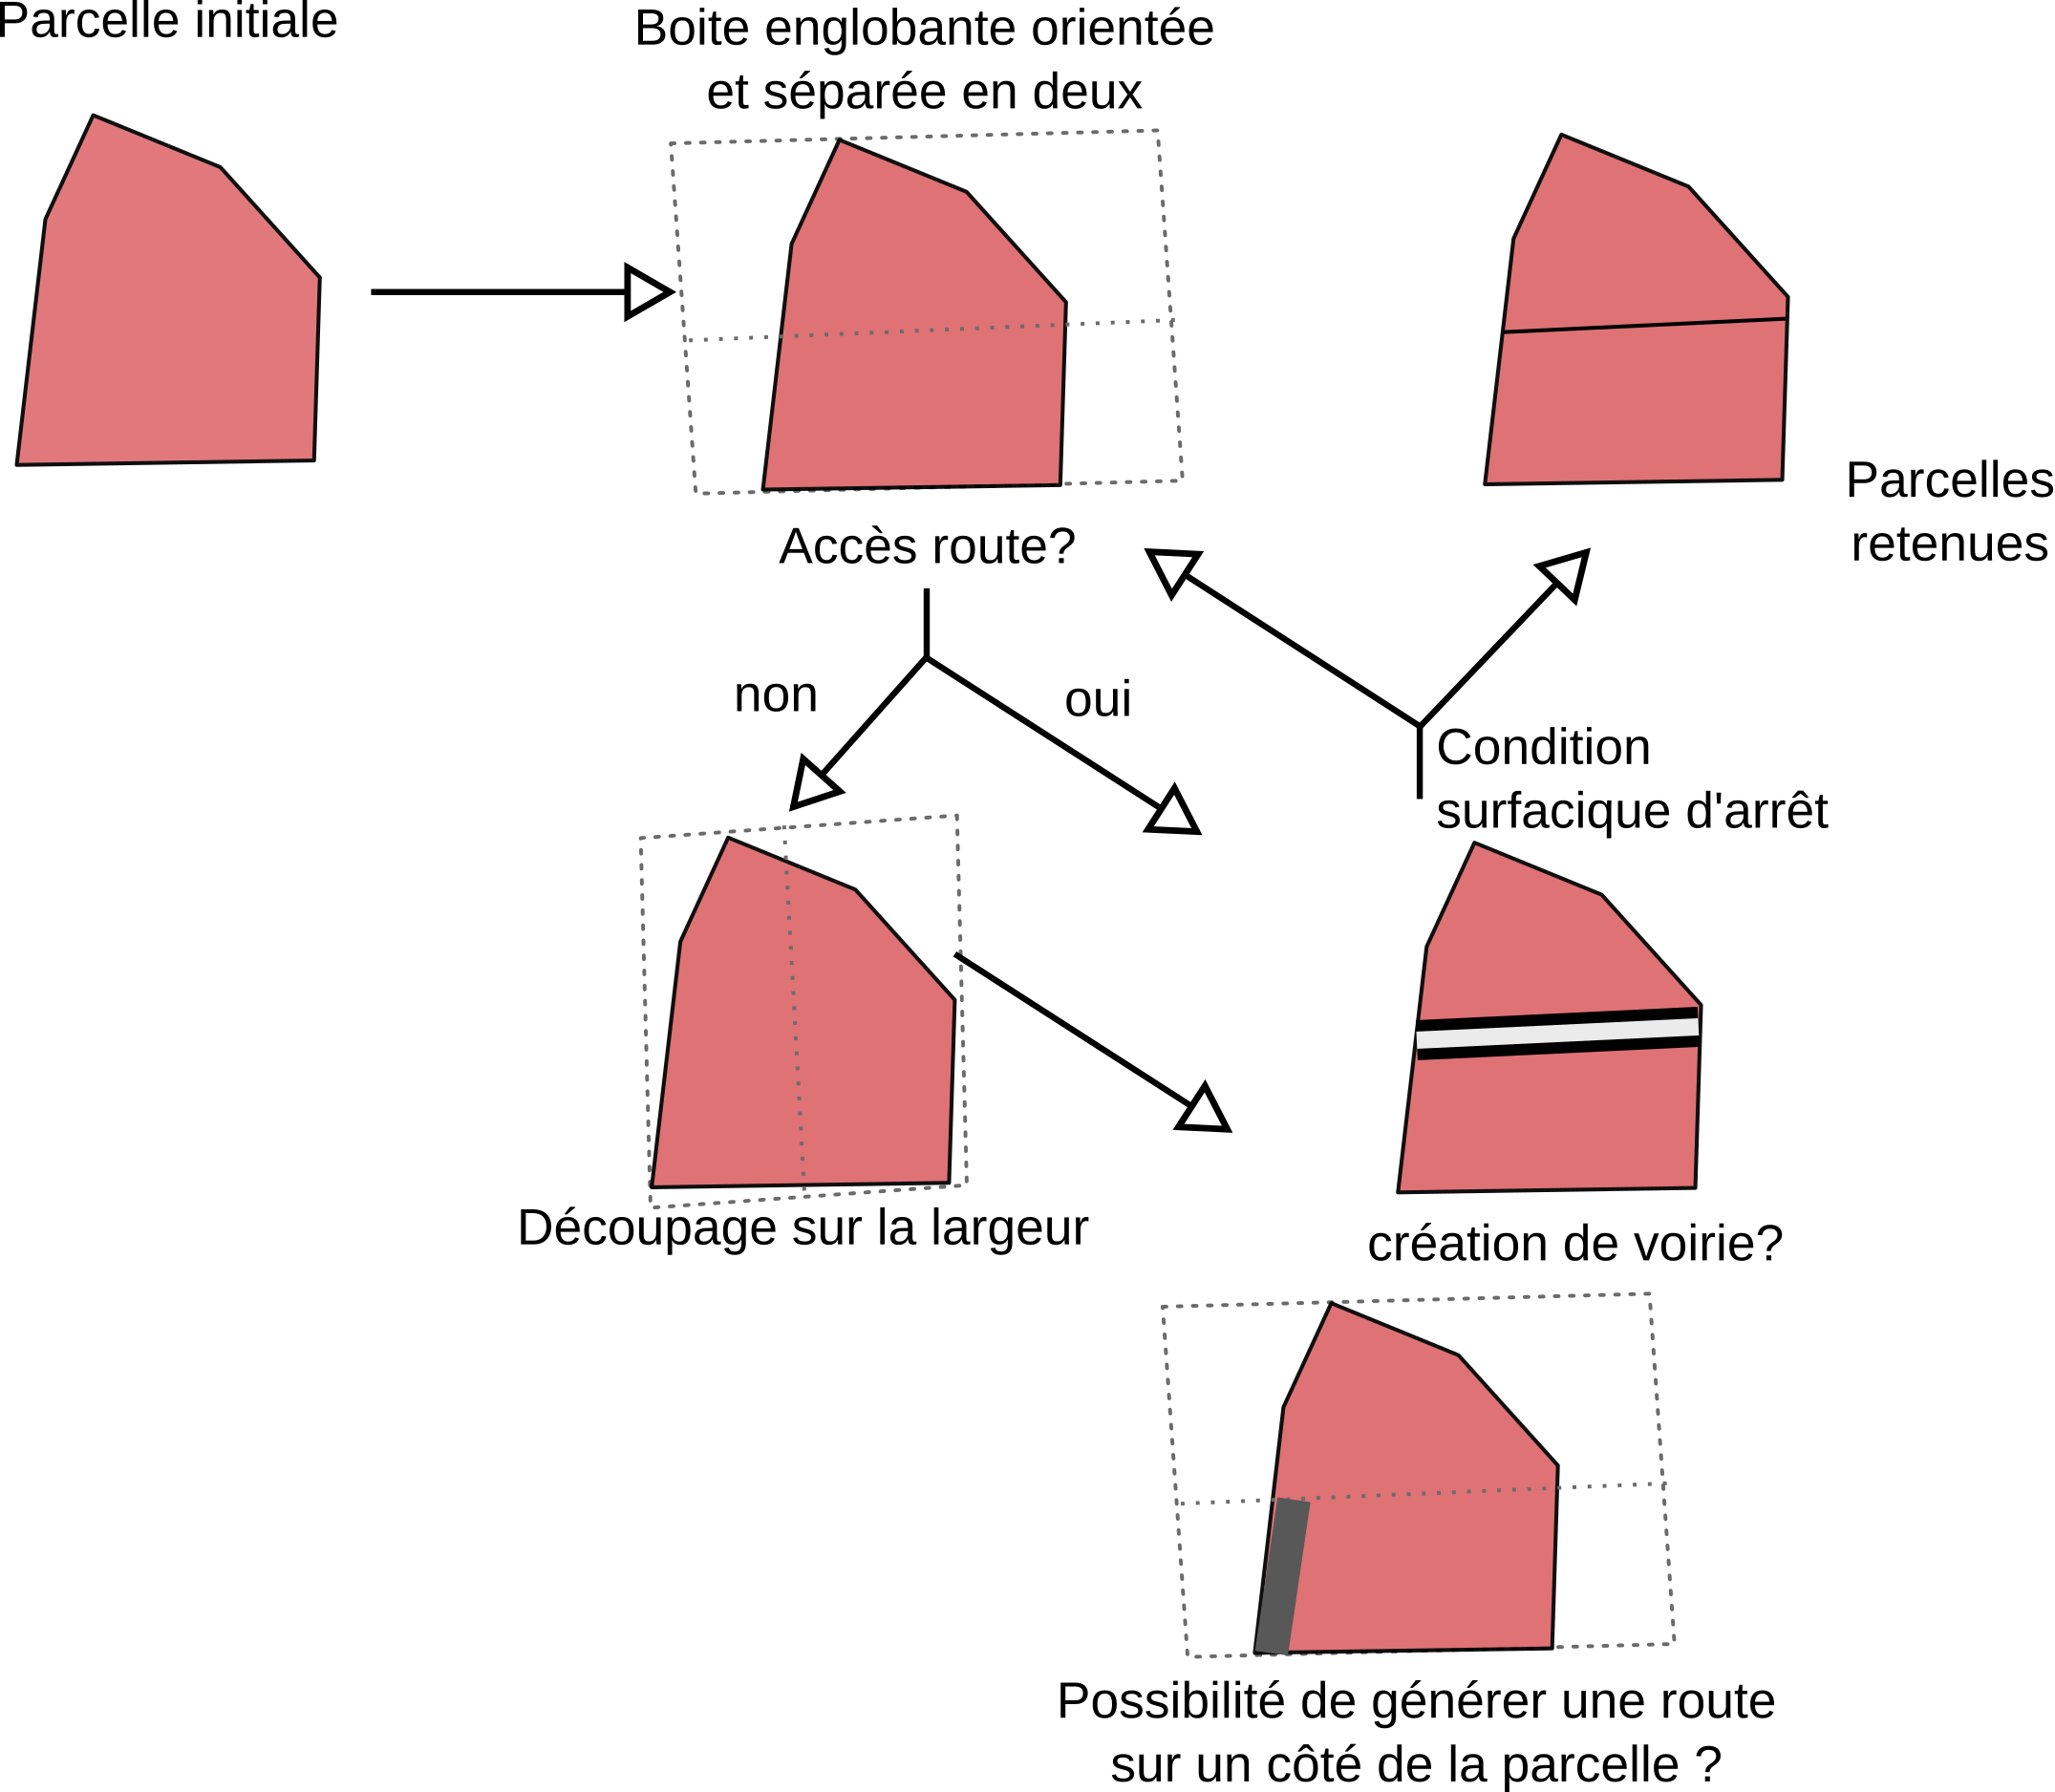
\includegraphics[width=9cm]{Images/decompositionParcelle-prez-apports.png}}}
\end{frame}
	
\begin{frame}<1>[label=PM]
	\frametitle{Algorithmes de recomposition parcellaire}
	\begin{itemize}
		\item \alert<1>{Densification}
		\item \alert<2>{Recomposition parcellaire totale}
		\item \alert<2>{Recomposition parcellaire partielle}
	\end{itemize}
\end{frame}

\begin{frame}{Densification}
 	\centering{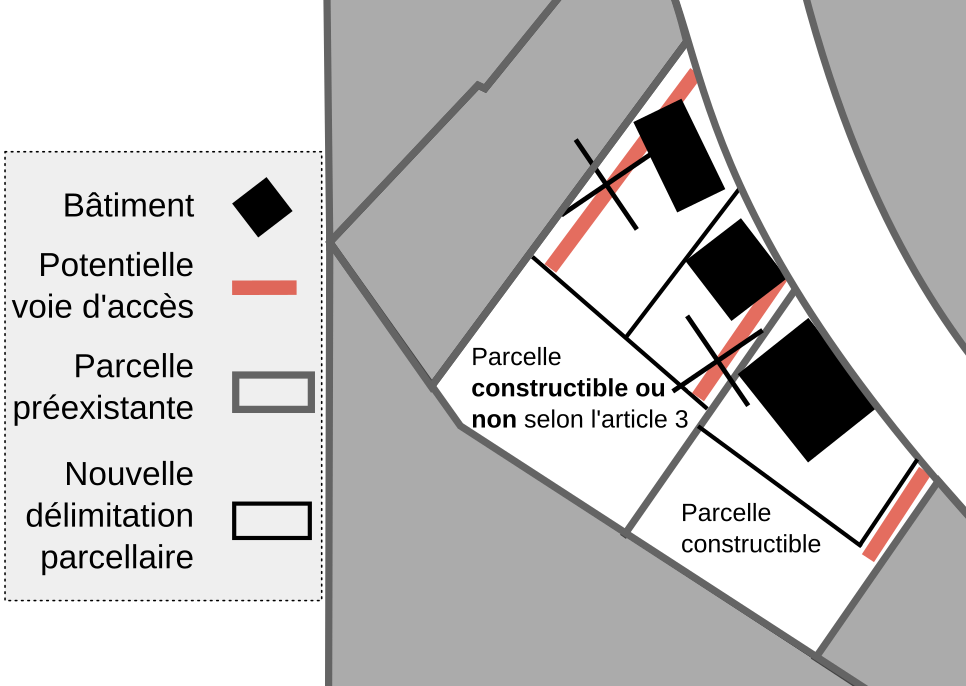
\includegraphics[width=9cm]{Images/splitParcelU.png}}
\end{frame}

\againframe<2>{PM}

\begin{frame}{Recomposition parcellaire totale}
 	\centering{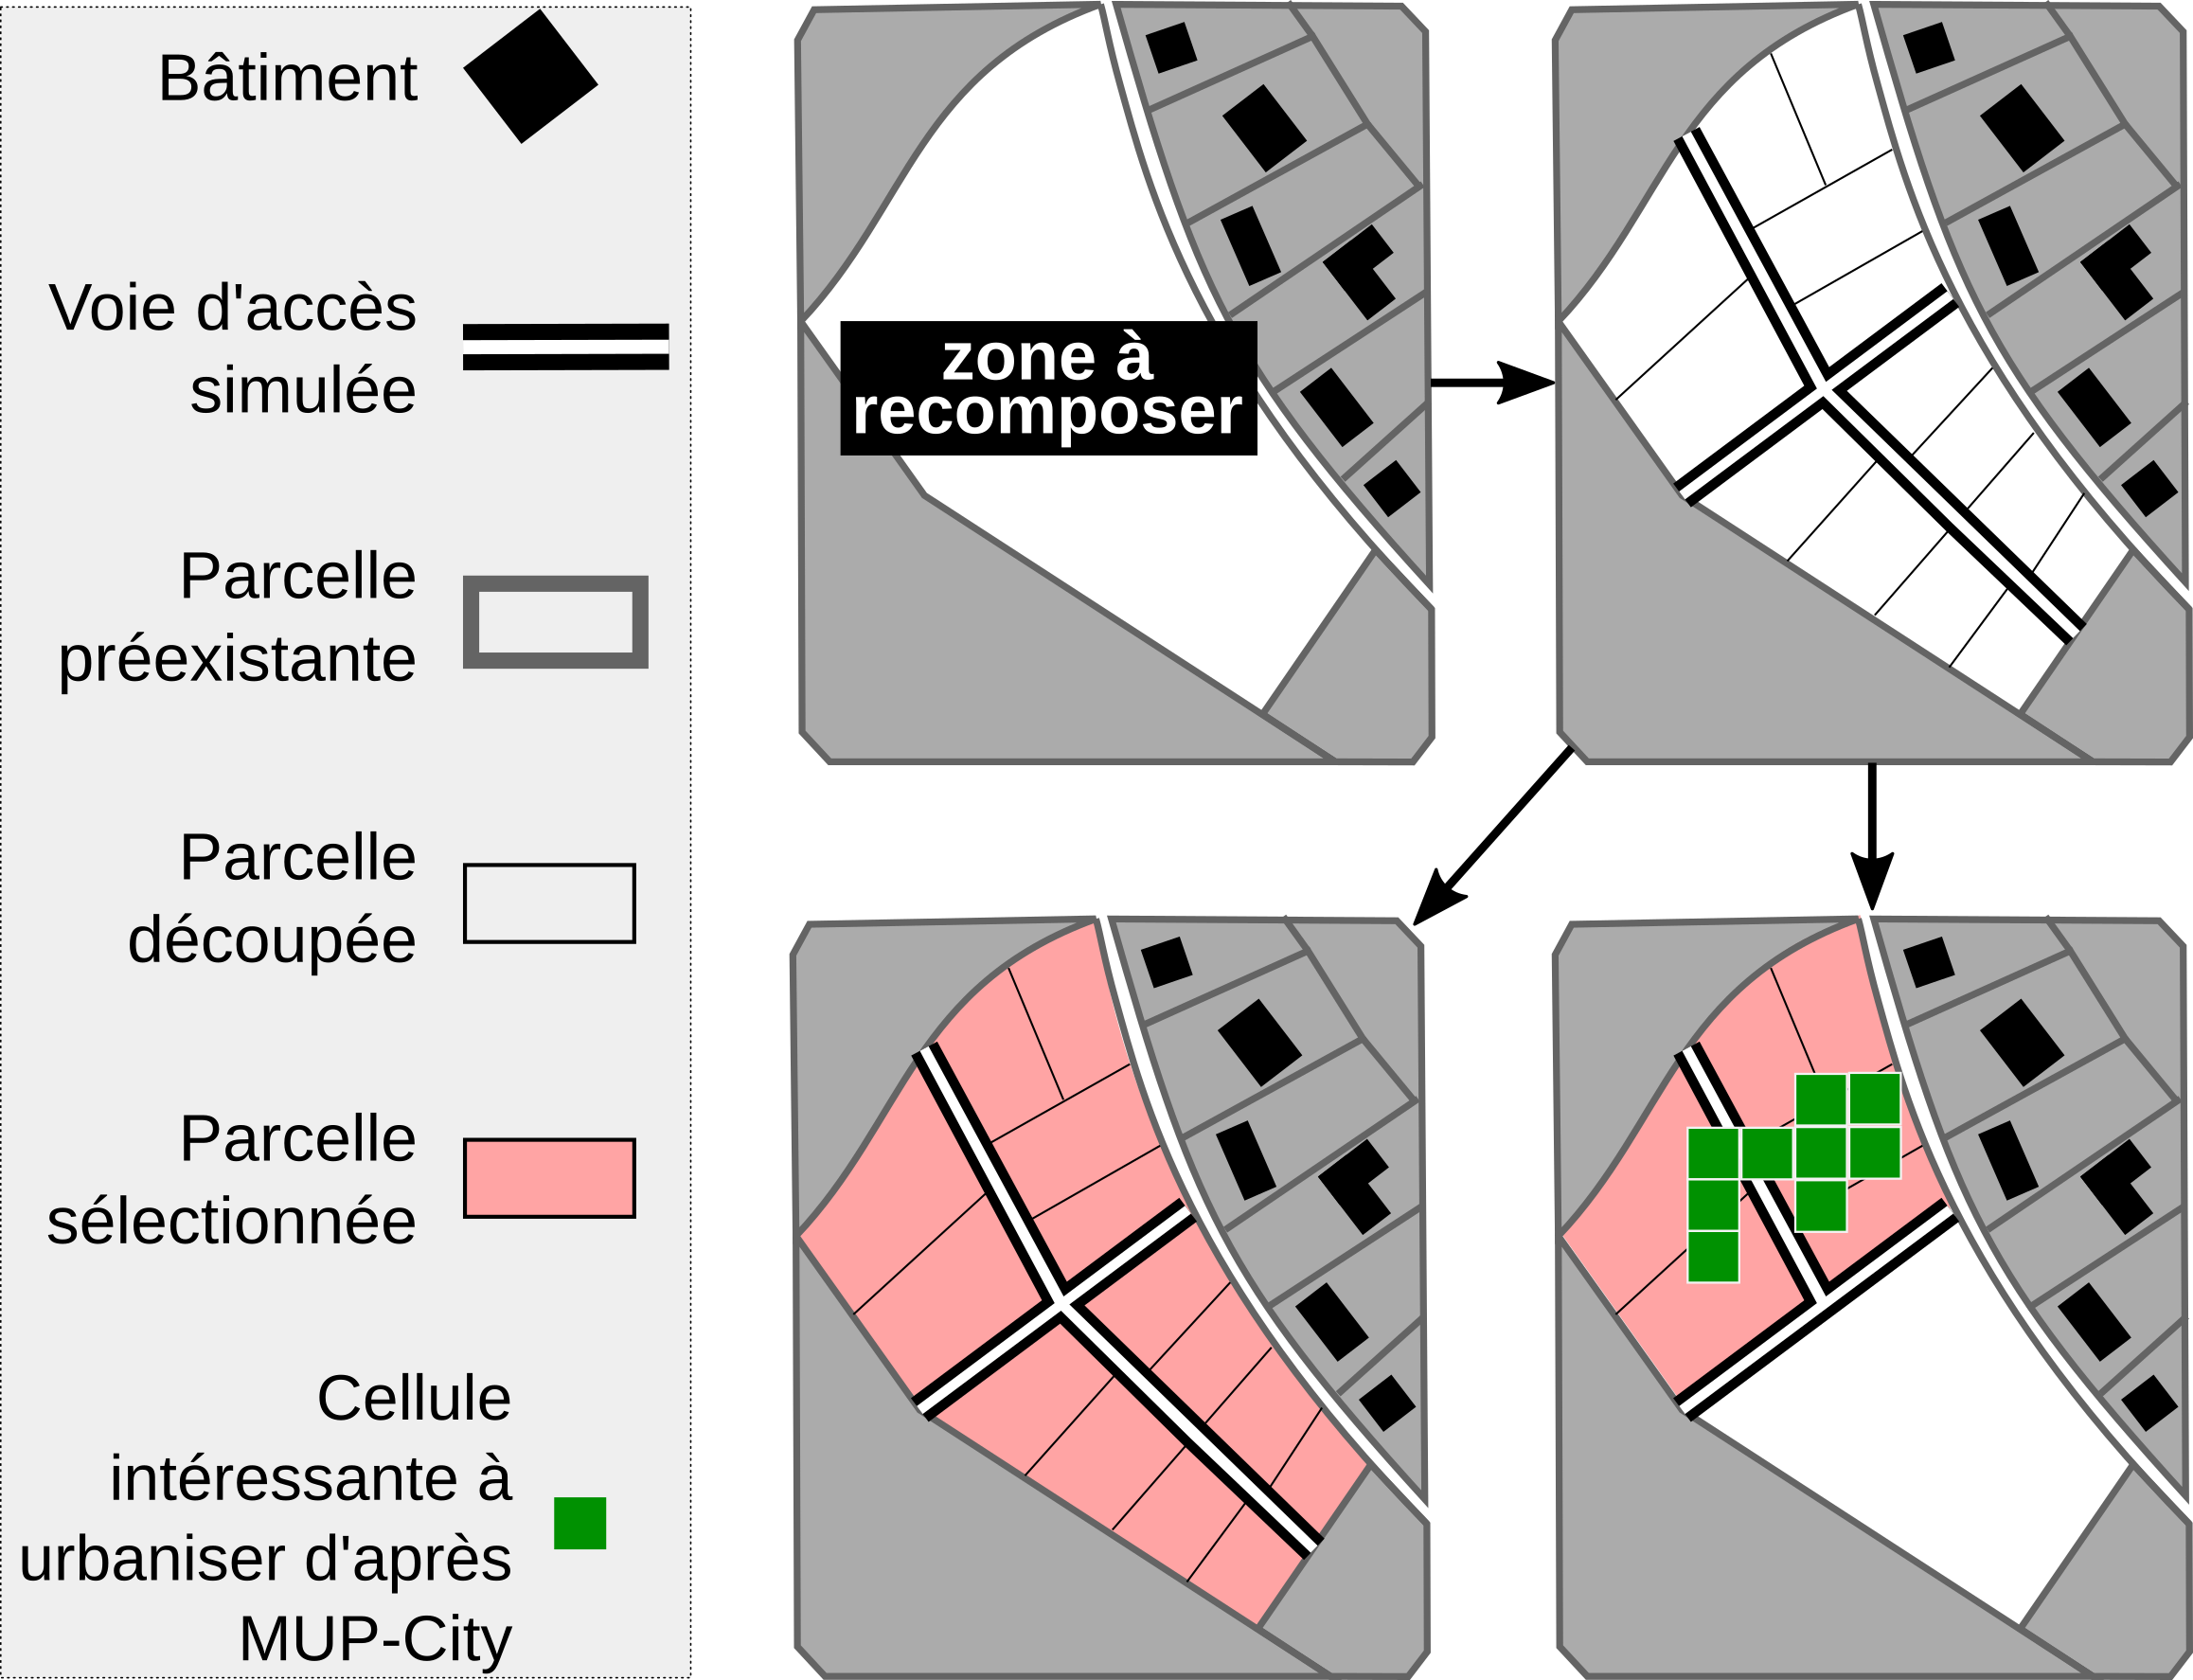
\includegraphics[width=9.5cm]{Images/splitParcelZone-prez.png}}
\end{frame}

%validation du module? 

\section[SimPLU3D]{SimPLU3D et la simulation de bâtiments}

\begin{frame}{Présentation de SimPLU3D}
	\centering{\textbf{SimPLU3D}}
	\begin{itemize}
		\item Génère un ensemble de bâtiments selon
		\begin{itemize}
			\item les \textbf{contraintes réglementaires}
			\item une forme prédéterminée
		\end{itemize}
		\item Optimise certains paramètres afin de poursuivre différents \textbf{objectifs de construction}
		\item Simule le comportement d'agents constructeurs
	\end{itemize} 
	\centering{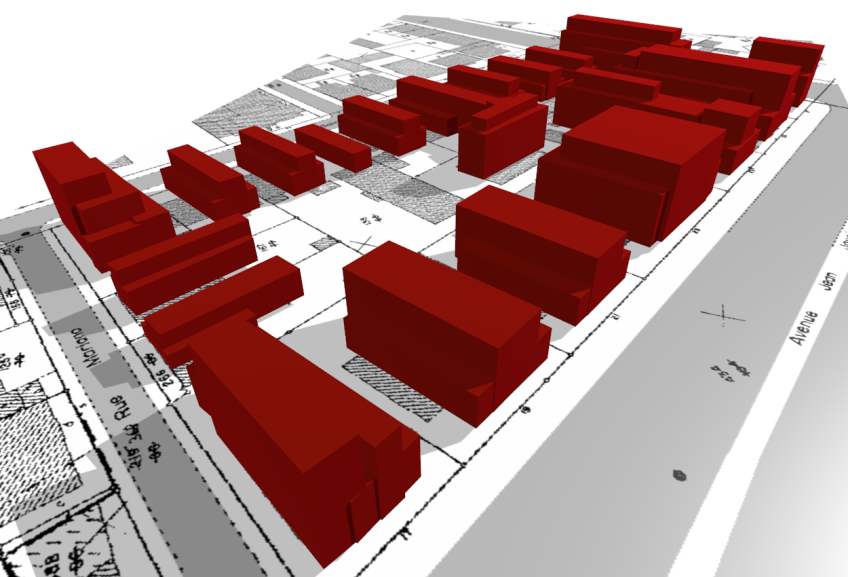
\includegraphics[width=5.5cm]{Images/SimpluOutput.png}}
\end{frame}

\begin{frame}{Formes prédéterminées des bâtiments}
	\begin{block}{}
		Adapter la \textbf{forme des bâtiments} simulés aux secteurs %approche prospective et non exploratoire
		\\
		Cinq types de bâtiments proposés~:
	\end{block}
	\only<1>{\textbf{Maison isolée}\\
		\begin{block}{}
		\centering{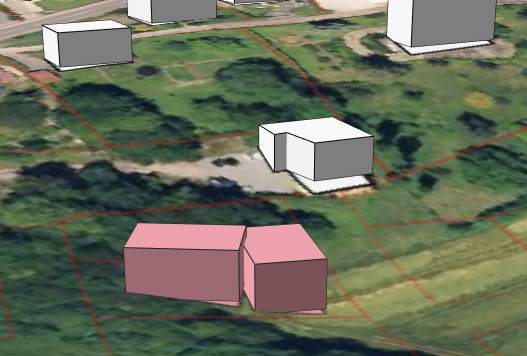
\includegraphics[width=6.5cm]{Images/detachedHouse.png}}
		\\
		{\footnotesize $[5-30]$ logements }	
	\end{block}}
	\only<2>{\textbf{Pavillon de lotissement}\\
	\begin{block}{}
		\centering{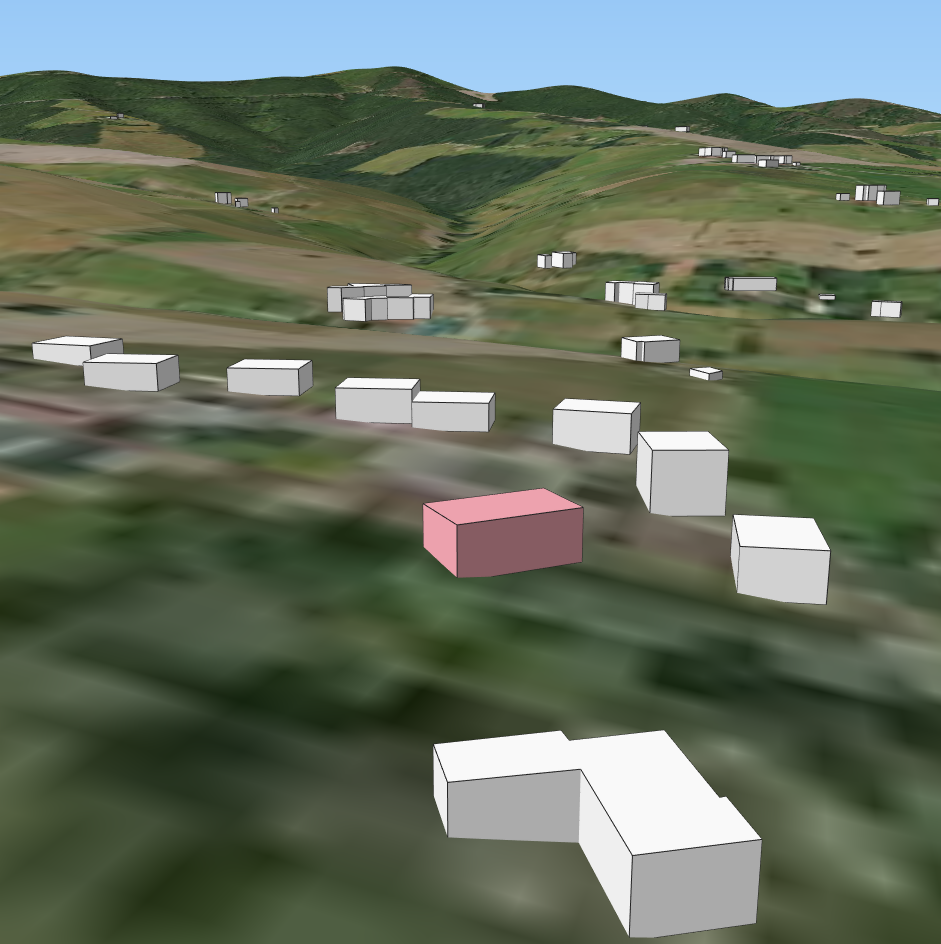
\includegraphics[width=4.5cm]{Images/smallBlock.png}}
		\\
		{\footnotesize logement individuel}	
	\end{block}}
	\only<3>{\textbf{Immeuble d'habitat intermédiaire}
	\begin{block}{}
		\centering{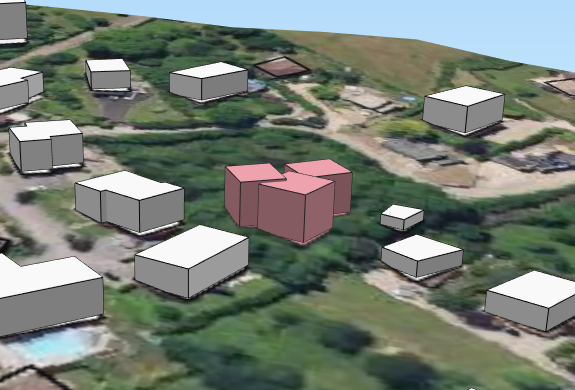
\includegraphics[width=6.5cm]{Images/multiFamilyHouse.png}}
		\\
		{\footnotesize $[2-9]$ logements}	
	\end{block}}
	\only<4>{\textbf{Petit immeuble collectif}\\
		\begin{block}{}
		\centering{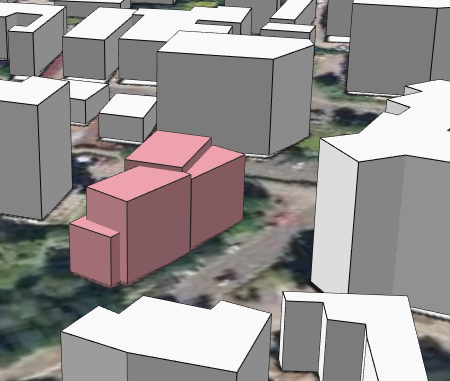
\includegraphics[width=5.5cm]{Images/smallBlockFlat.png}}
		\\
		{\footnotesize $[5-30]$ logements}	
		\end{block}}

	\only<5>{\textbf{Immeuble collectif de taille moyenne}\\
		\begin{block}{}
		\centering{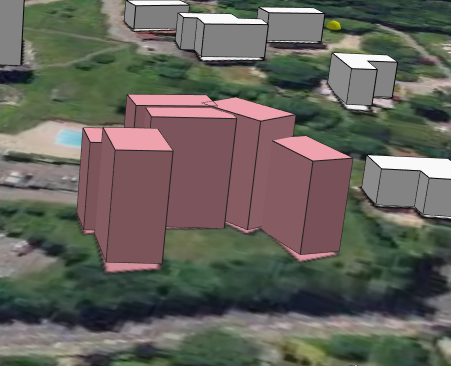
\includegraphics[width=5.5cm]{Images/midBlockFlat.png}}
		\\
		{\footnotesize $[30-60]$ logements}	
	\end{block}}
\end{frame}

\begin{frame}{Estimation de logements}
	\begin{itemize}
		\item Tirage aléatoire d'une classe d'appartements
		\item Surface paramétrable de ces classes
		\item Distribution paramétrable des logements dans l'immeuble 
	\end{itemize}
\end{frame}

\begin{frame}{Apports internes à ArtiScales}
	\centering{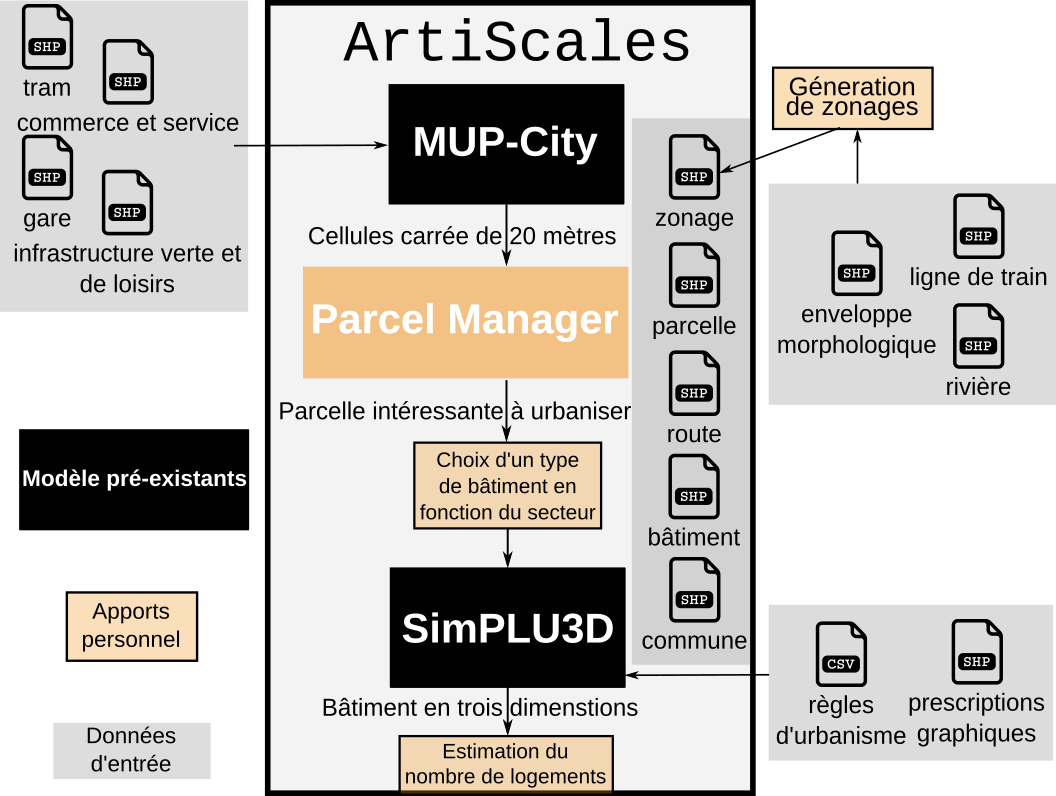
\includegraphics[width=11cm]{Images/schemGen-prez-apports}}
\end{frame}


\section{Validation du modèle MUP-City}

\begin{frame}{MUP-City: analyse de variabilité}
	\begin{block}{}
		{\small Les résultats de simulations de MUP-City sont très variables (Tannier 2012, Fremont 2015)}
		\only<1>{\begin{block}{}
			\centering{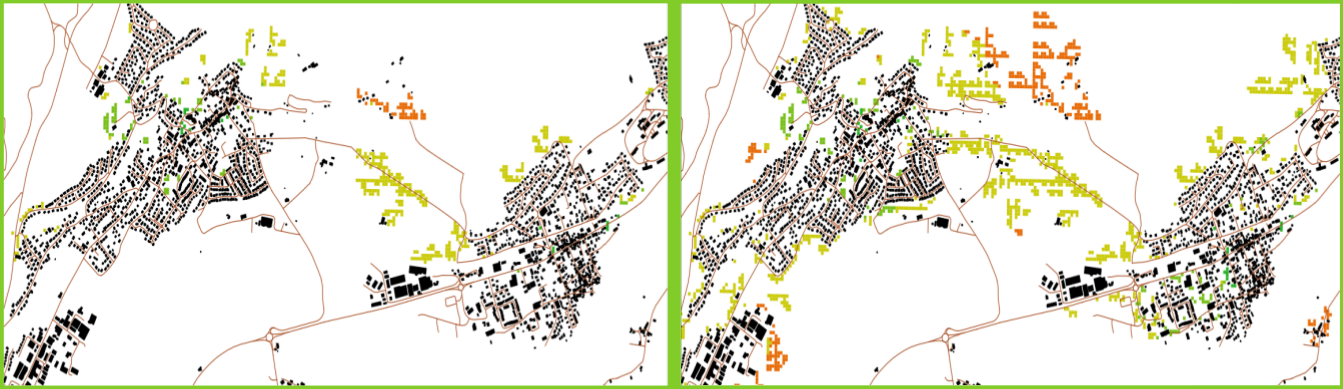
\includegraphics[width=10cm]{Images/ex-sorties-mup2.png}}
			\\
			{\footnotesize exemple de variations stochastiques des résultats de MUP-City}
		\end{block}}
	\end{block}
	\uncover<2->{\begin{block}{}
	{\Large 	\textbf{Analyse de variabilité}}
	\end{block}}
	\uncover<3->{\begin{block}{Principes}
			\footnotesize
				Analyser la variation des résultats de simulation d'un modèle\\
				Rechercher de la source de cette variabilité
		\end{block}}
	\uncover<4->{\begin{block}{Objectifs}
		\footnotesize 
			\textbf{Fiabilité} des résultats de simulation\\
			Sélection de \textbf{configurations résidentielles} à exploiter
		\end{block}}
	\uncover<5>{\begin{block}{Approche}
			\footnotesize
			Étude des paramètres dits \alert{techniques}\\
			Étude des paramètres dits \alert{scénaristiques}
		\end{block}}

\end{frame}

\begin{frame}<1>[label=parScen]
\frametitle{MUP-City: paramètres scénaristiques}
	\begin{enumerate}
		\item \alert<1>{Intensité du développement résidentiel}
		\item<2-> \alert<2>{Uniformité du développement résidentiel}
		\item<3-> \alert<3>{Pondération des règles additionnelles d'aménagement}
		\item<4> \alert<4>{Aggrégation des règles additionnelles d'aménagement}
	\end{enumerate}
\end{frame}

\begin{frame}{MUP-City : intensité du développement résidentiel}
\vspace{1cm}
\centering{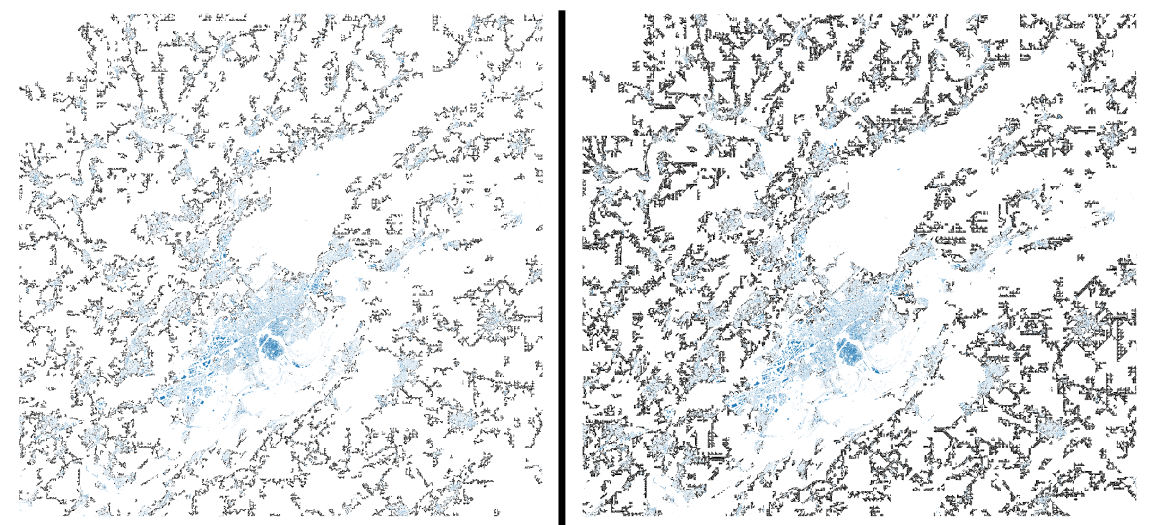
\includegraphics[width=11.5cm]{Images/MUP/Intens.png}\\
	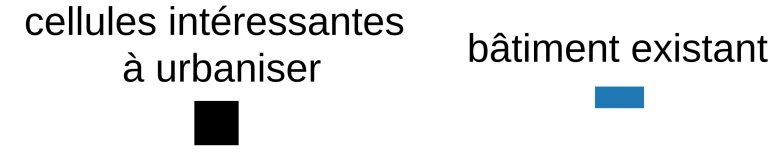
\includegraphics[width=4cm]{Images/MUP/legend.png}}
\\
{\footnotesize Exemples d'un scénario peu dense et d'un scénario modérément dense} %TODO ajouter légende
\end{frame}

\againframe<2>{parScen}

\begin{frame}{MUP-City : uniformité du développement résidentiel}
\vspace{1cm}
\centering{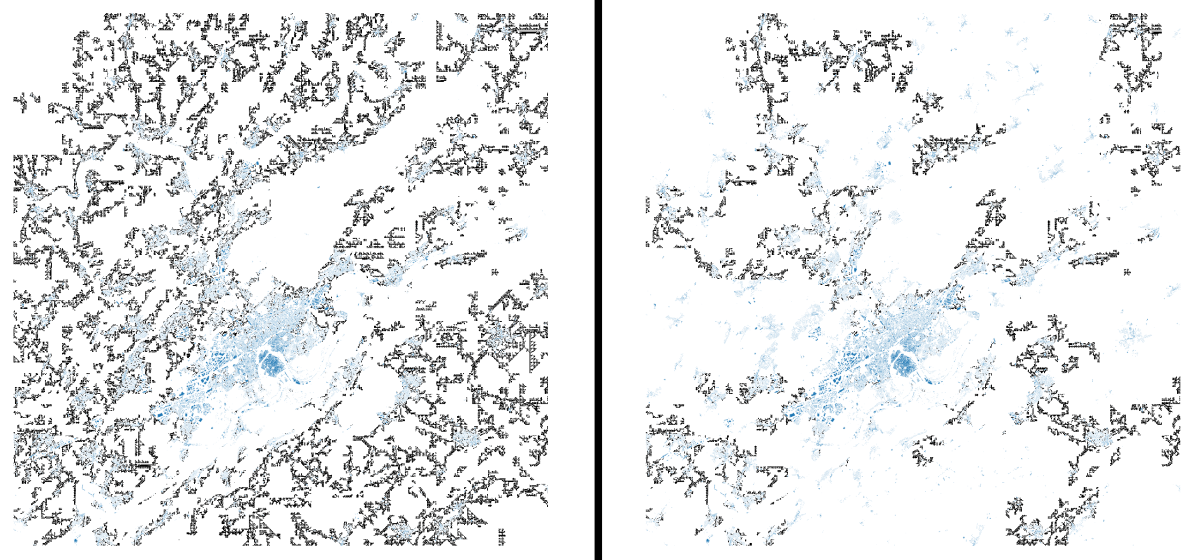
\includegraphics[width=11.5cm]{Images/MUP/Unif.png}\\
	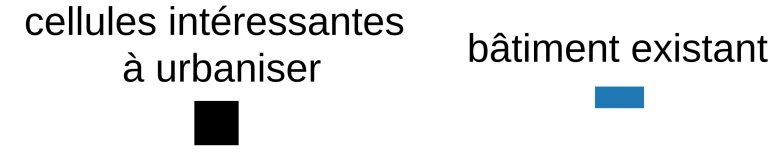
\includegraphics[width=4cm]{Images/MUP/legend.png}}}
\\
{\footnotesize Exemples d'un scénario uniforme et d'un scénario contrasté}%TODO ajouter légende
\end{frame}

\againframe<3>{parScen}

\begin{frame}{MUP-City : orientation du développement résidentiel}
\vspace{1cm}
\centering{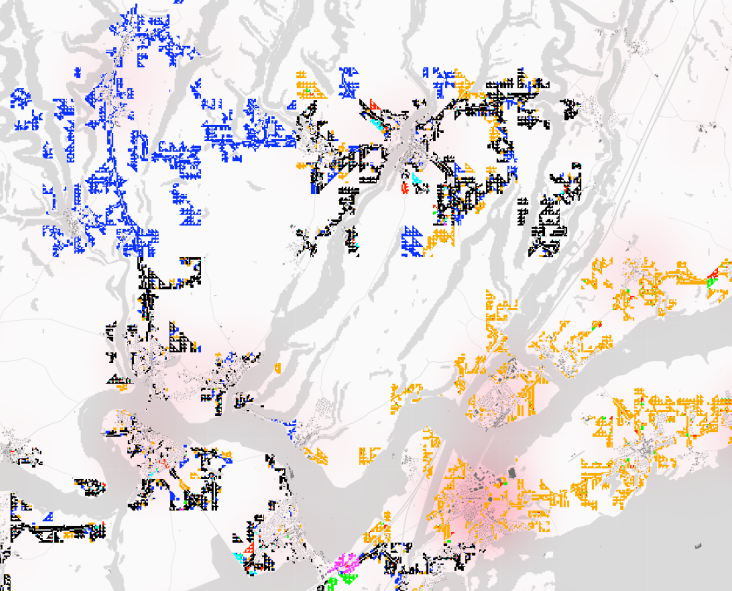
\includegraphics[width=8cm]{Images/MUP/Ahp.png}}
\\
{\footnotesize Exemple de différentes orientations poursuivies par le développement résidentiel}%TODO ajouter légende
\end{frame}

\againframe<4>{parScen}

\begin{frame}{MUP-City : caractère extensif ou non de l'extension résidentielle}
\vspace{1cm}
\centering{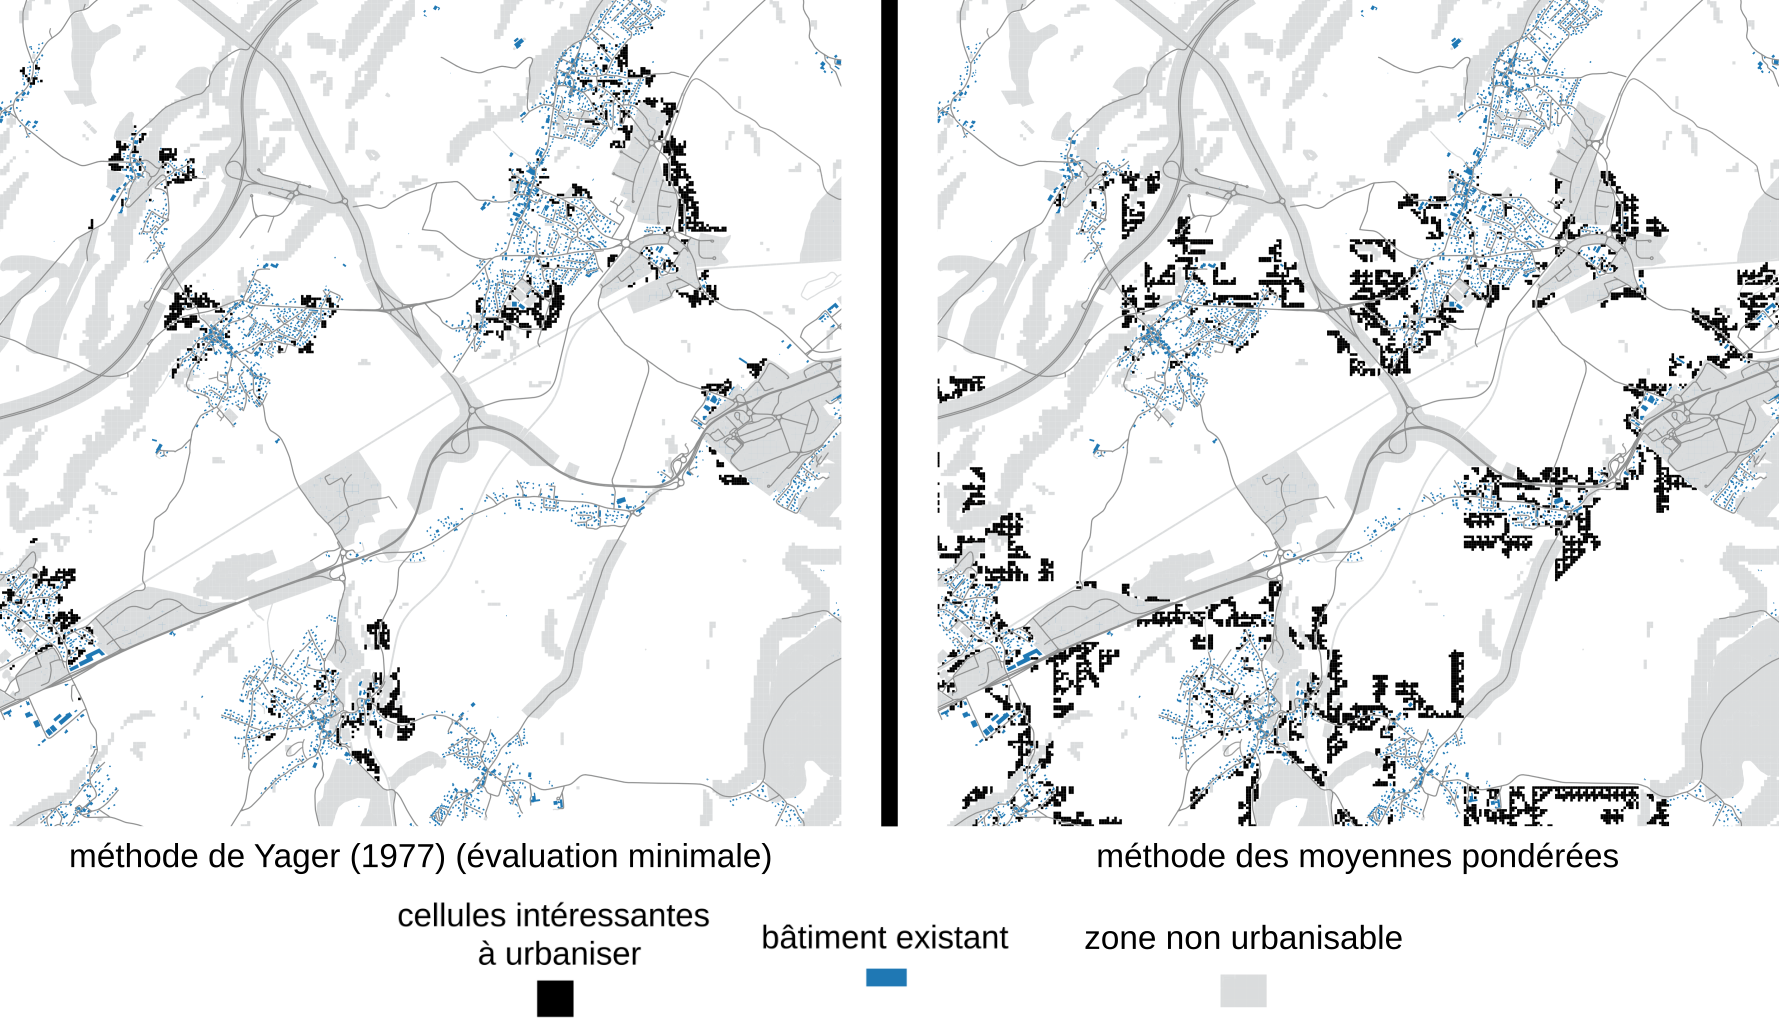
\includegraphics[width=12cm]{Images/MUP/illuYagMoy.png}} %TODO changer l'image + légende
%\centering{\includegraphics[width=11.5cm]{Images/MUP/Agreg.png}}

{\footnotesize exemple de différentes agrégations des règles additionnelles d'aménagement, résultant en un scénario sélectionnant des cellules uniformément intéressantes à urbaniser ou non}
\end{frame}

\begin{frame}{Validation de différentes configurations spatiales de MUP-City}
	\only<1>{Indicateurs utilisés
	\begin{itemize}
		\item Nombre de cellules selon et leurs localisation
		\item Correspondance aux objectifs de création de logements
		\item Dimension fractale, accessibilitée ... 
	\end{itemize}
	}
	\only<2>{\begin{block}{Scénario d'étalement résidentiel}
	\vspace{0.4cm}
		{\footnotesize Scénario de développement résidentiel \textbf{uniforme}, \textbf{peu intense} et \textbf{extensif}~:}
		\begin{block}{}
			\centering{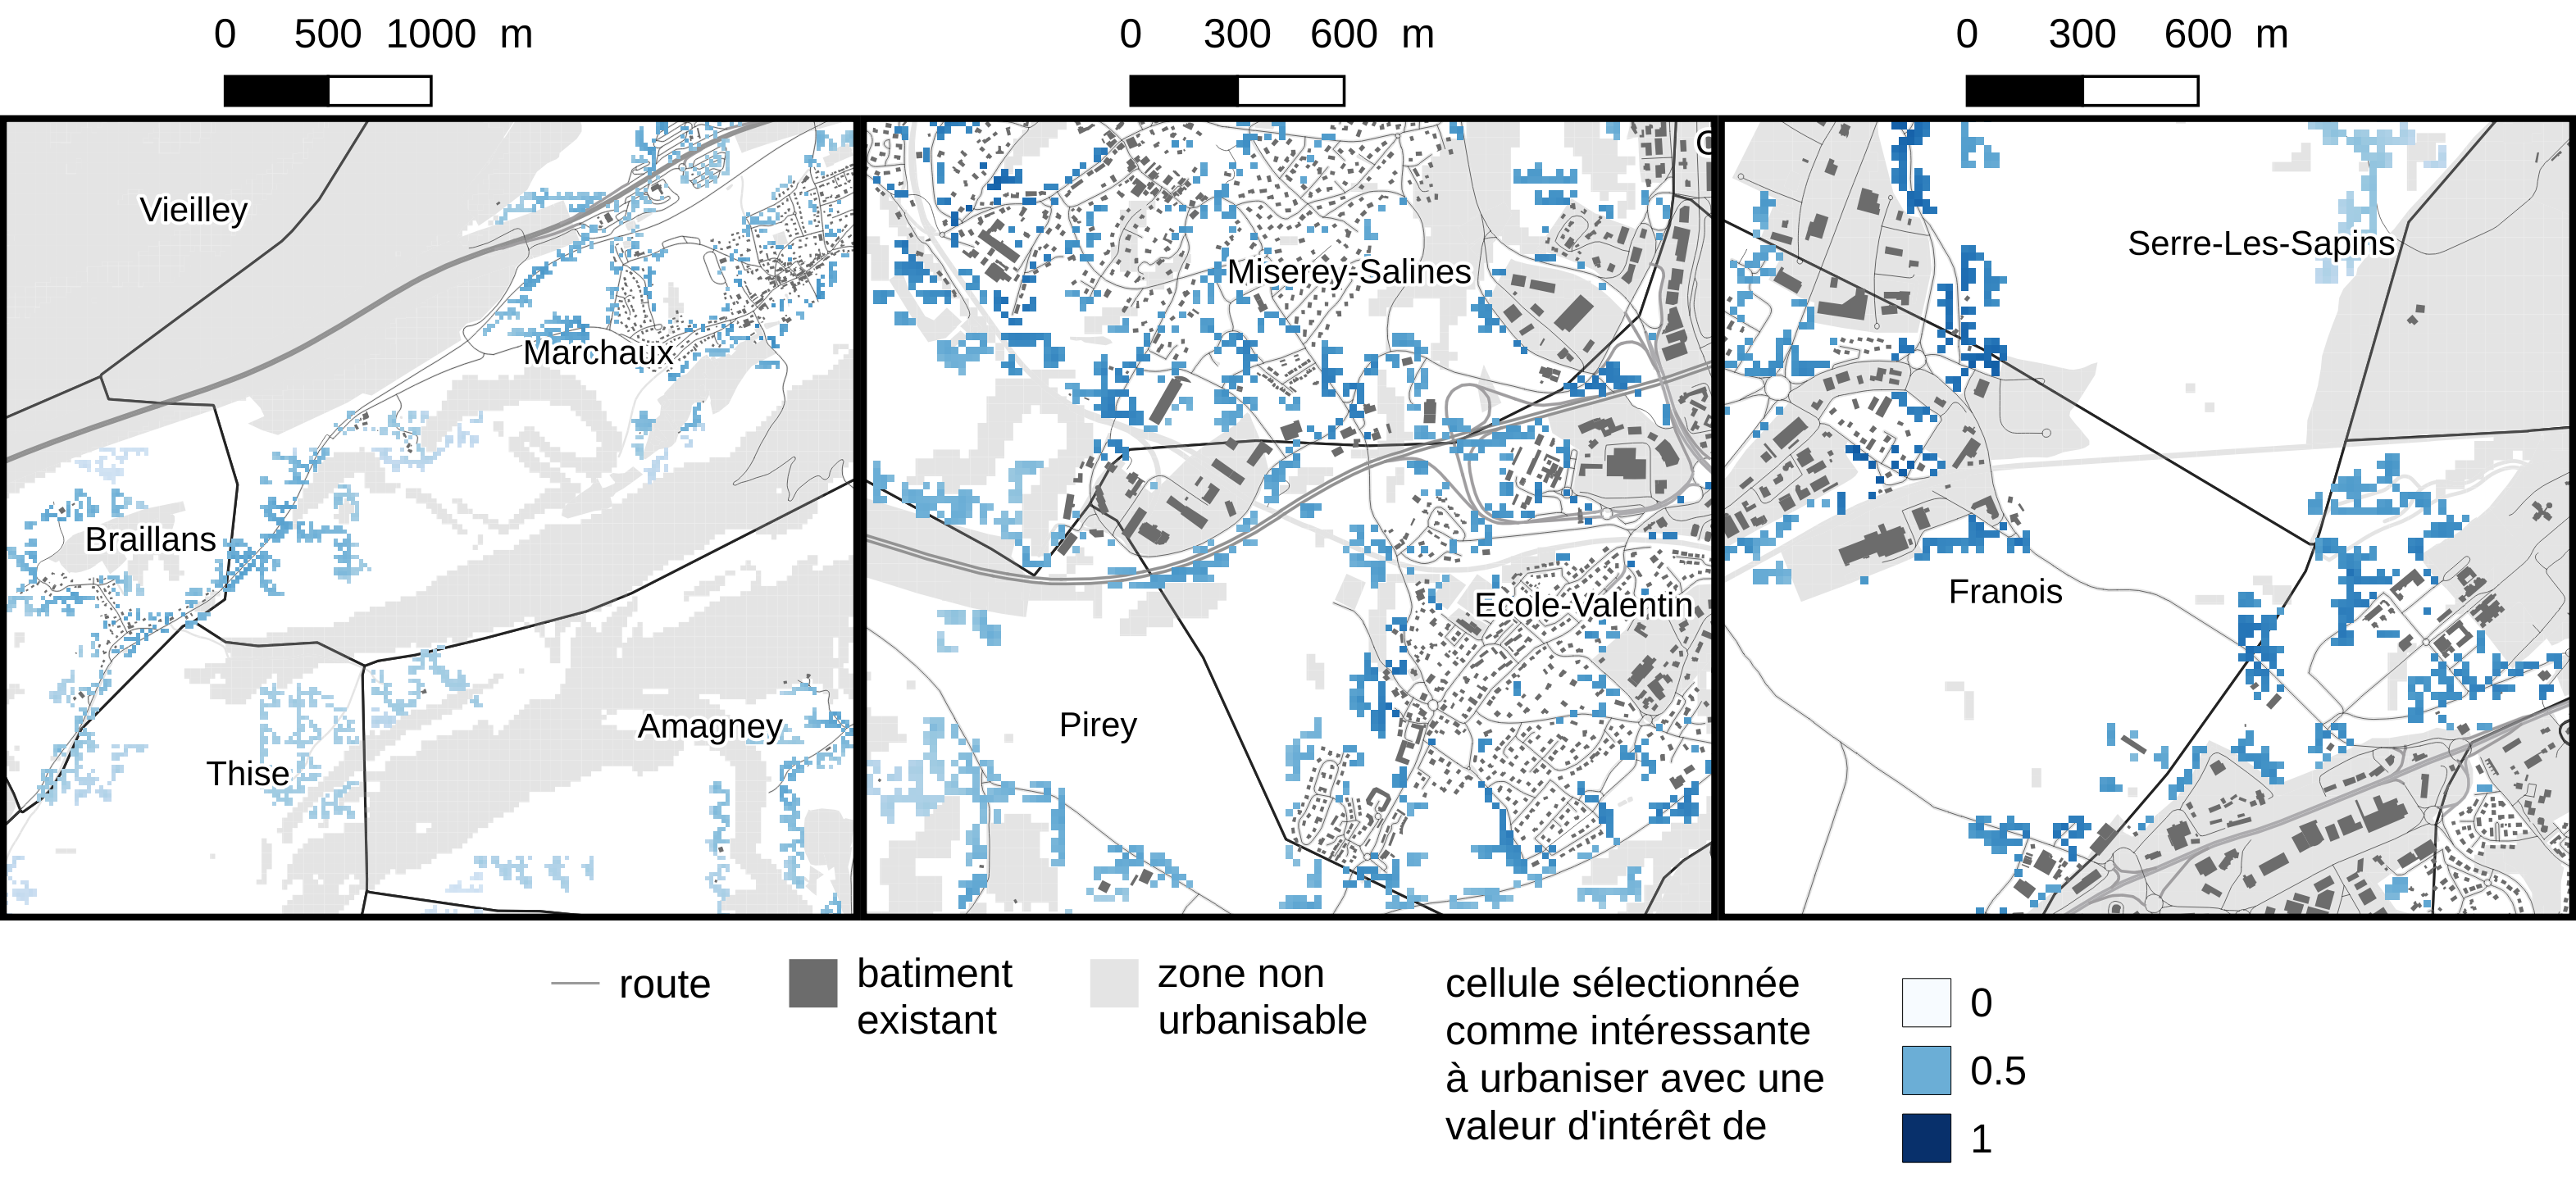
\includegraphics[width=11cm]{Images/MUP/ManuN5Bazomm.png}}
		\end{block}
	\end{block}}
	\only<3>{\begin{block}{Scénario d'extension résidentielle ciblée}
	\vspace{0.4cm}
		{\footnotesize Scénario de développement résidentiel \textbf{contrasté}, \textbf{intense} et \textbf{extensif}~:}
		\begin{block}{}
			\centering{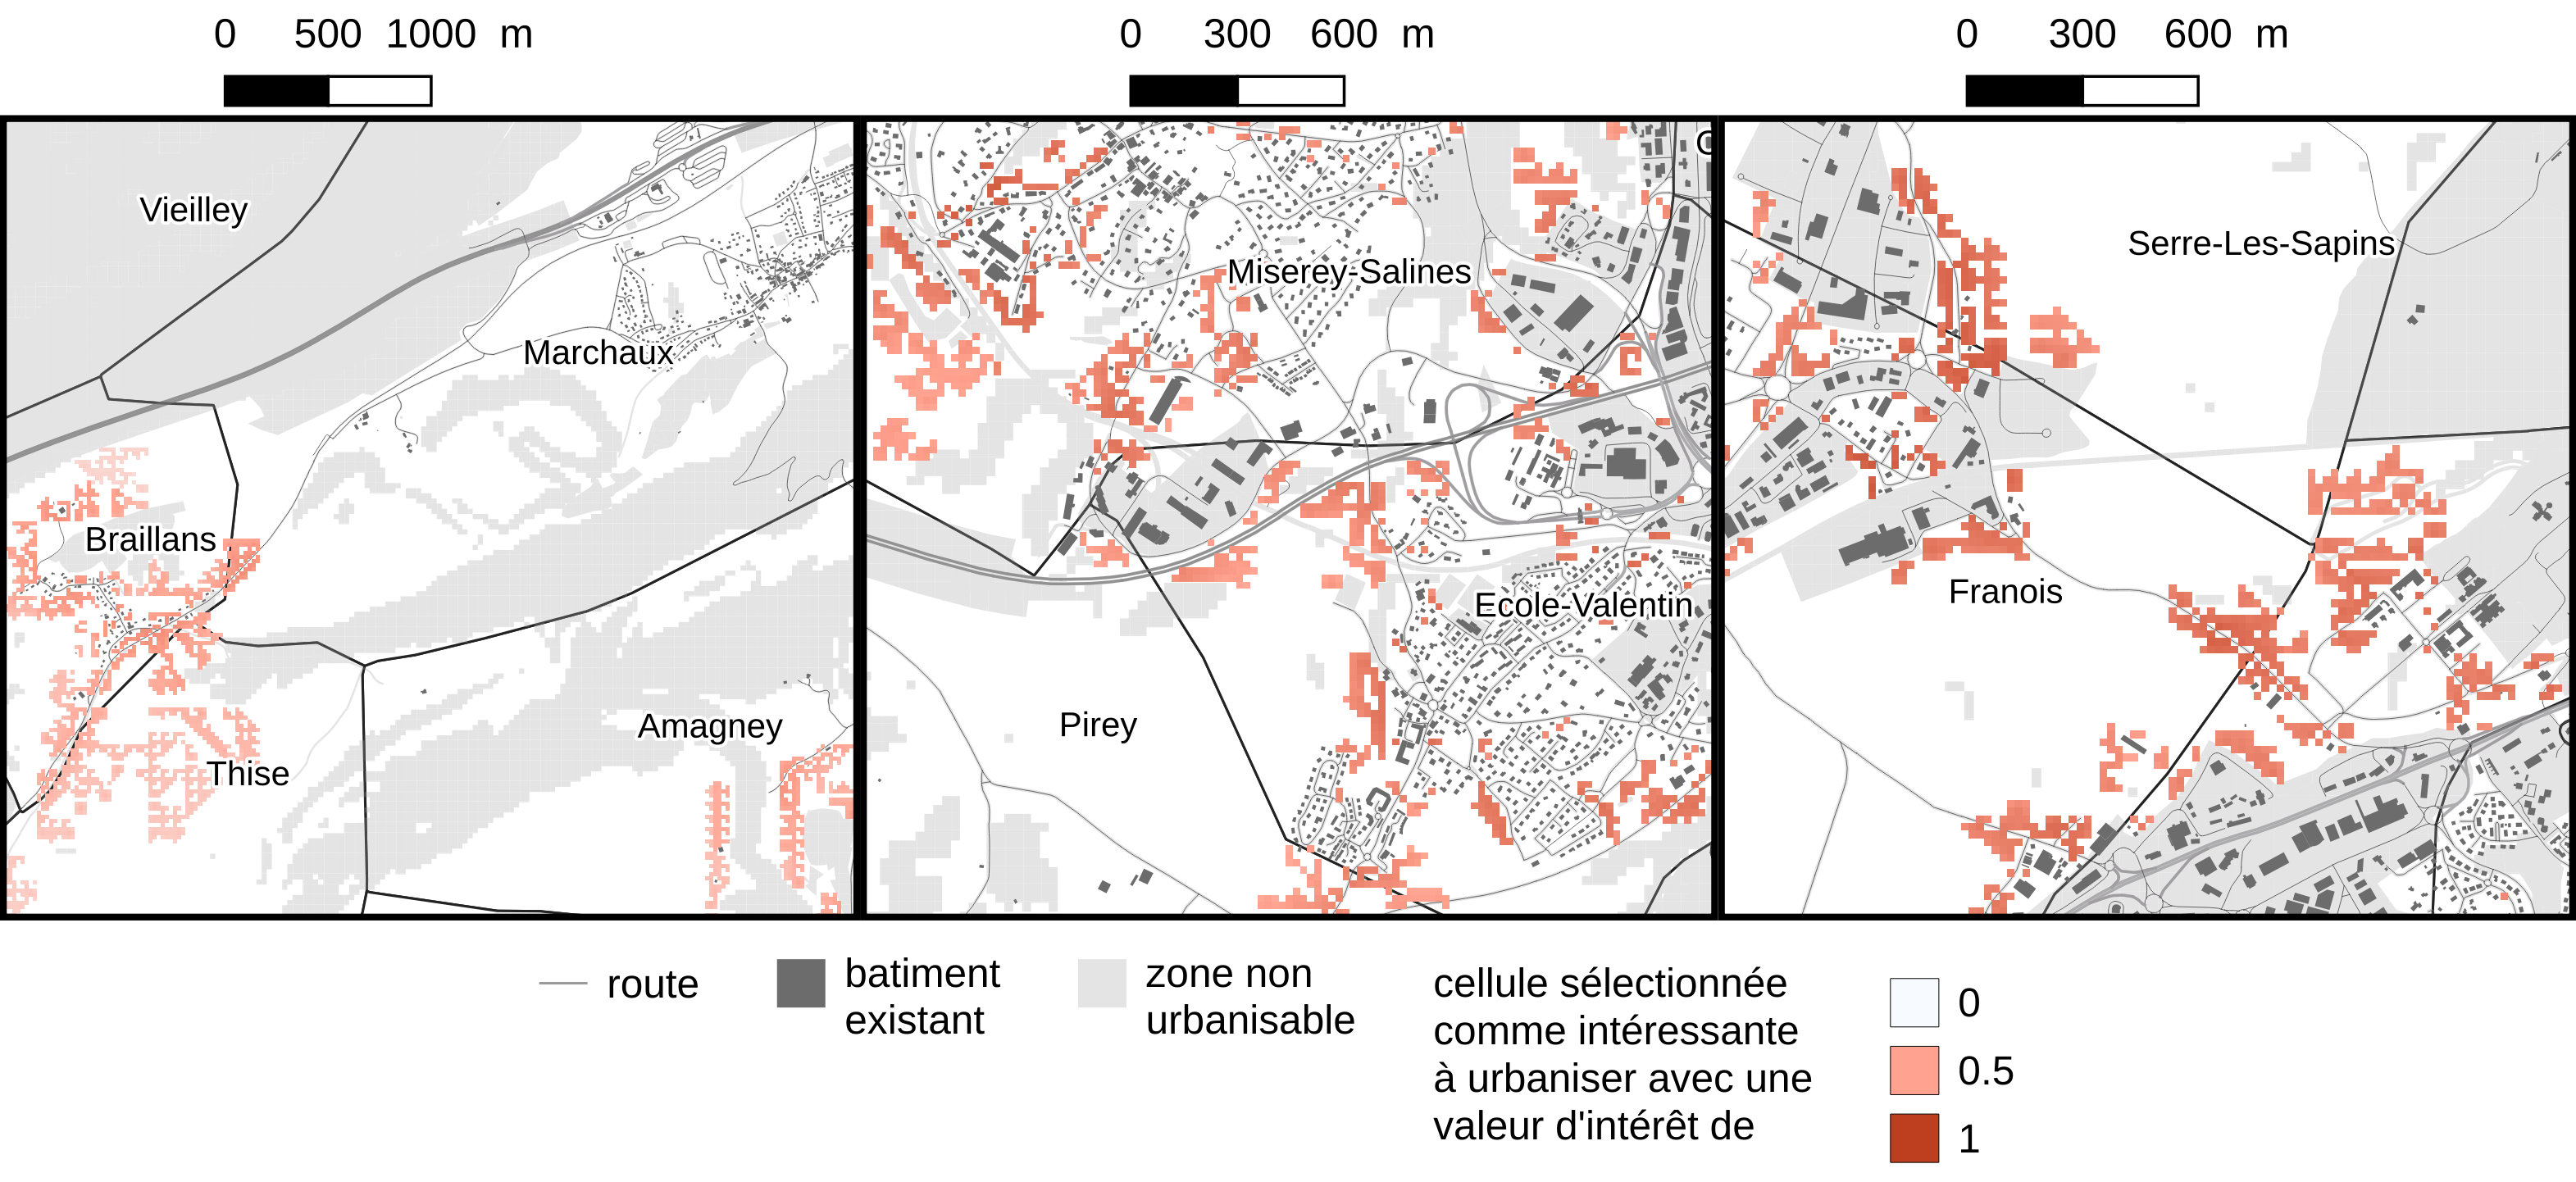
\includegraphics[width=11cm]{Images/MUP/ManuN6Stzomm.png}}
		\end{block}
	\end{block}}
	\only<4>{\begin{block}{Scénario d'intensification de la densité résidentielle}
	\vspace{0.4cm}
		{\footnotesize	Scénario de développement résidentiel \textbf{peu extensif}, \textbf{uniforme} et \textbf{très intense}~:}
		\begin{block}{}
			\centering{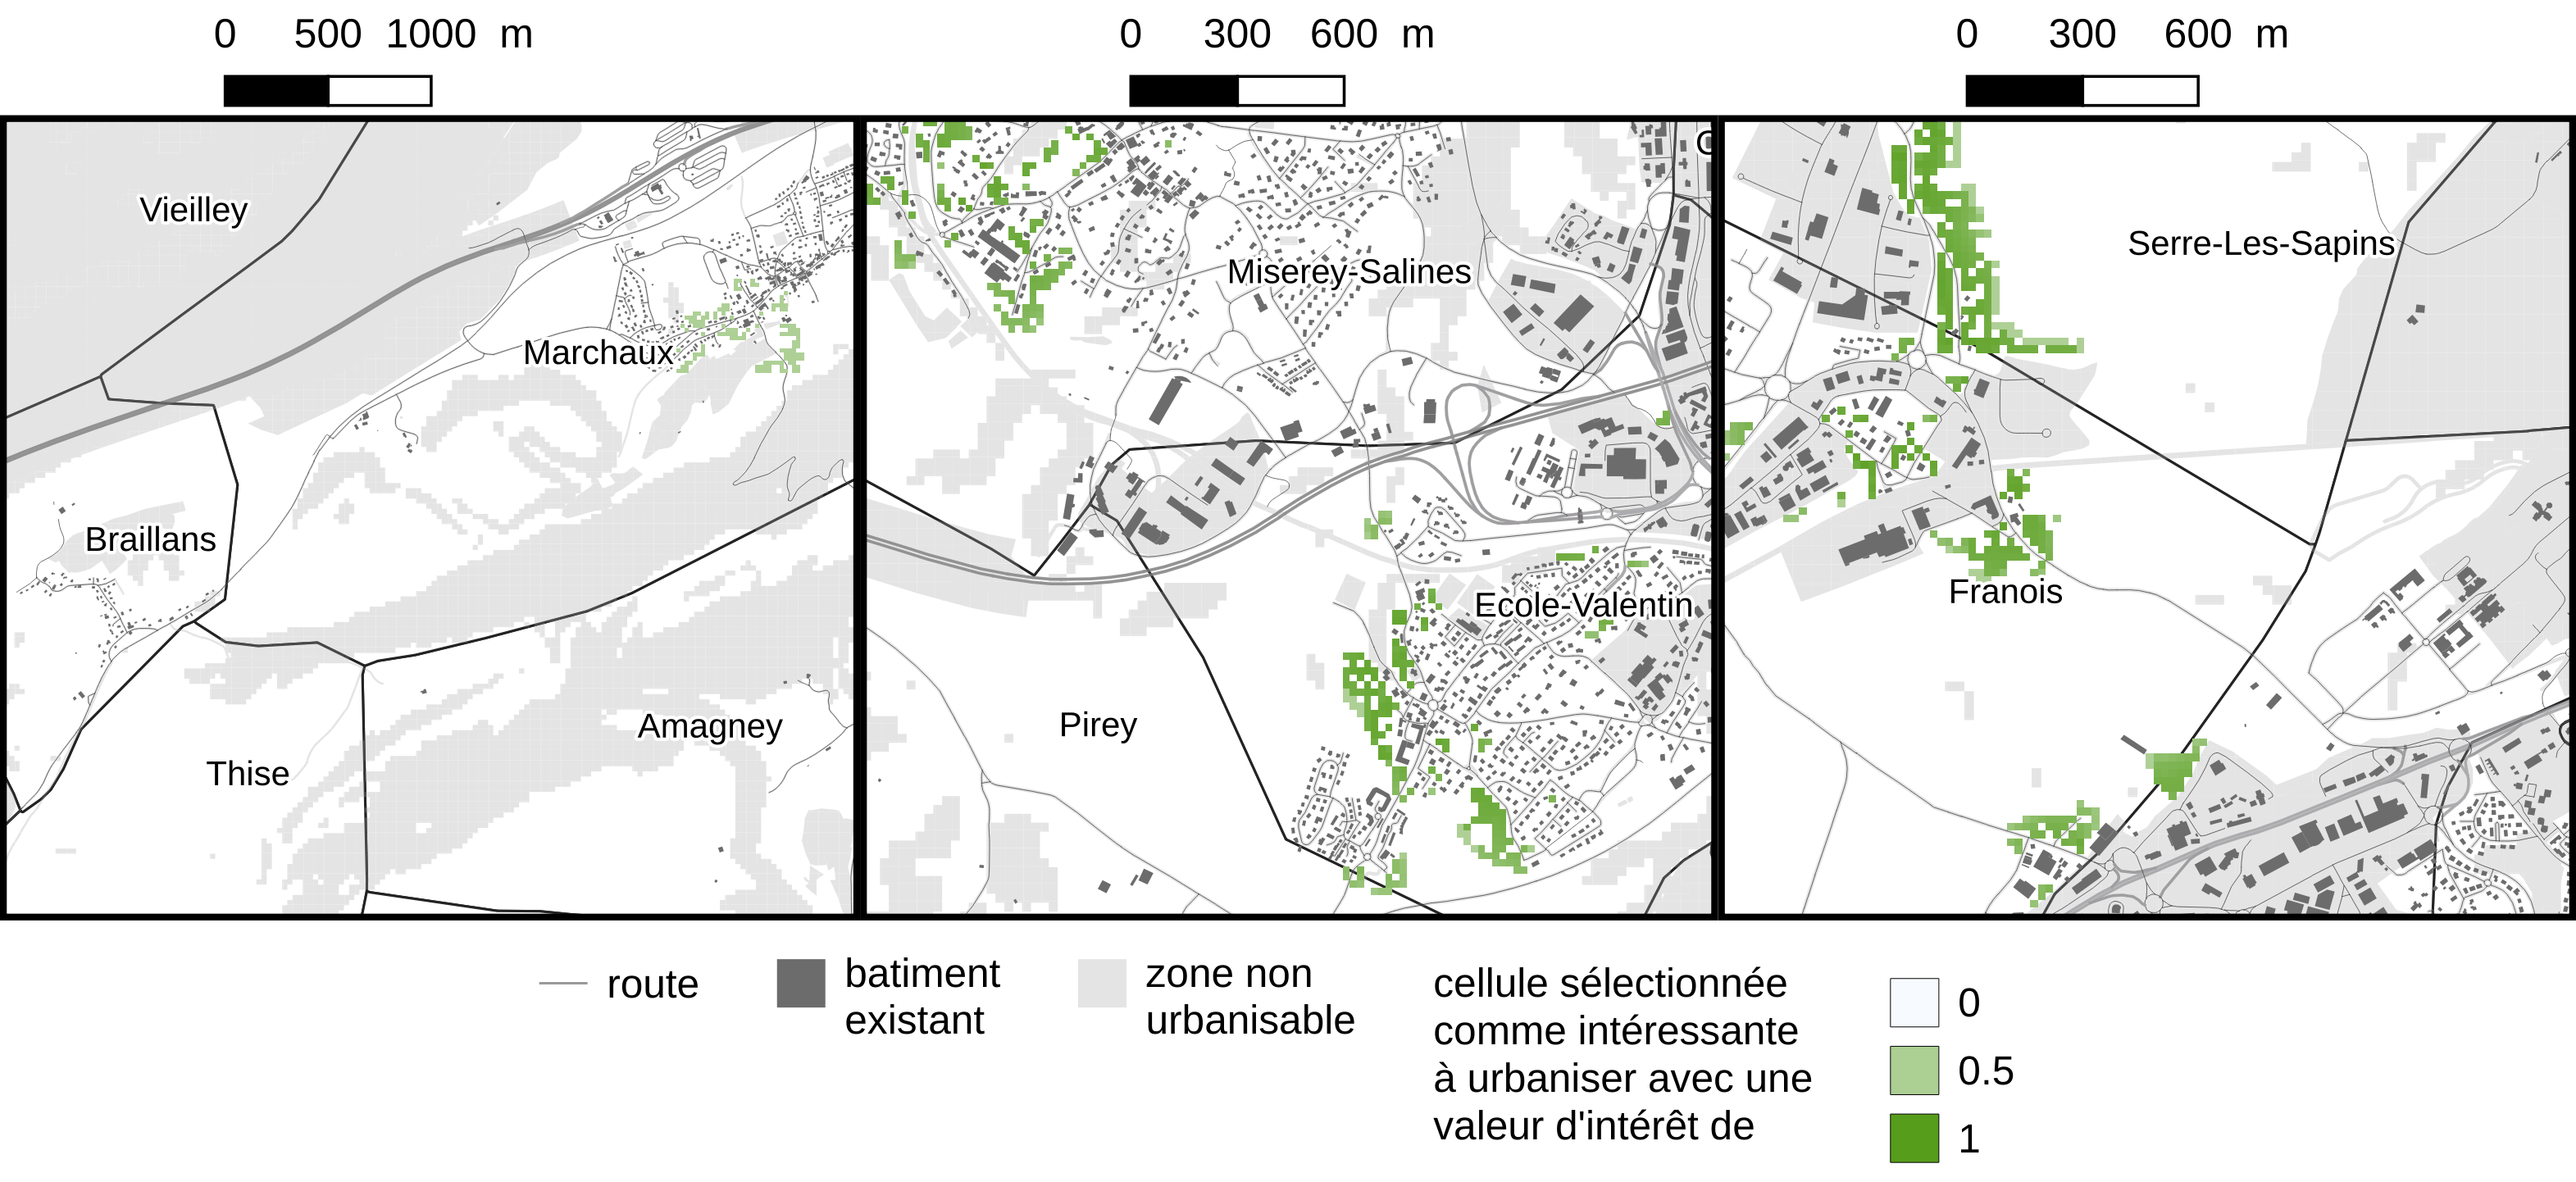
\includegraphics[width=11cm]{Images/MUP/ManuN7Yagzomm.png}}
		\end{block}
	\end{block}}
\end{frame}

\begin{frame}{MUP-City : Paramètres techniques}
	Différentes catégories de \textbf{paramètres techniques}~:\\
	\begin{itemize}
		\item Graine du générateur de nombres pseudo-aléatoires
		\item Définition et méthode de préparation des jeux de données d'entrée
		\item Position de la grille de décomposition
		\item Taille des cellules en sortie
	\end{itemize}
\end{frame}

\begin{frame}{MUP-City : variabilité due aux paramètres techniques}
	\only<1>{
		Combinaison de types de paramètres 
		\\
		\textbf{Indicateurs}~:
		\begin{itemize}
			\item Réplication de la sélection des cellules 
			\item Intérêt des cellules à être urbanisées
			\item Surface sélectionnée
		\end{itemize}
	}
	\only<2>{
		\begin{block}{Scénario d'\textbf{étalement résidentiel}}
			\begin{itemize}
				\item variable selon la position éloignée de la grille de décomposition
				\item peu variable selon d'autre paramètres techniques
			\end{itemize}
		\end{block}
	}
	\only<3>{
		\begin{block}{Scénario d'\textbf{extension résidentielle ciblée}}
			\begin{itemize}
				\item Potentiellement très variable du fait du \textbf{caractère aléatoire}
				\item Très variable selon la taille des cellules
				\item Variable selon la position éloignée de la grille de décomposition
			\end{itemize}
		\end{block}	
	}
	\only<4>{
		\begin{block}{Scénario d'\textbf{intensification de la densitée résidentielle}}
			\begin{itemize}
				\item Très variable du fait du \textbf{caractère aléatoire}
				\item Localement très sensible à la position de la grille de décomposition
			\end{itemize}
		\end{block}	
	}
\end{frame}

\begin{frame}{MUP-City : conclusion de l'analyse de variabilité}
	\begin{block}{Conclusion}
		La variation de certains paramètres d'entrée n'ont pas les mêmes effets sur les sorties
		\\
		Détections d'indicateurs pertinents à optimiser
	\end{block}
	\uncover<2->{\begin{block}{}
		Plusieurs configurations résidentielles simulées
		\\
		Différents scénarios de développement résidentiel
		\\
		Différentes variantes de ces scénarios
	\end{block}}
	\uncover<3>{\begin{block}{}
		\textbf{Validation thématique de ces scénarios}
	\end{block}}
\end{frame}


\section{Validation du Parcel Manager}

\begin{frame}{Validation du Parcel Manager}
	Application de l'algorithme sur l'ensemble de la zone d'étude et comparaisons de caractéristiques
	\\
	Comparaisons avec certaines opérations spéciales d'aménagement
	\begin{block}{}
		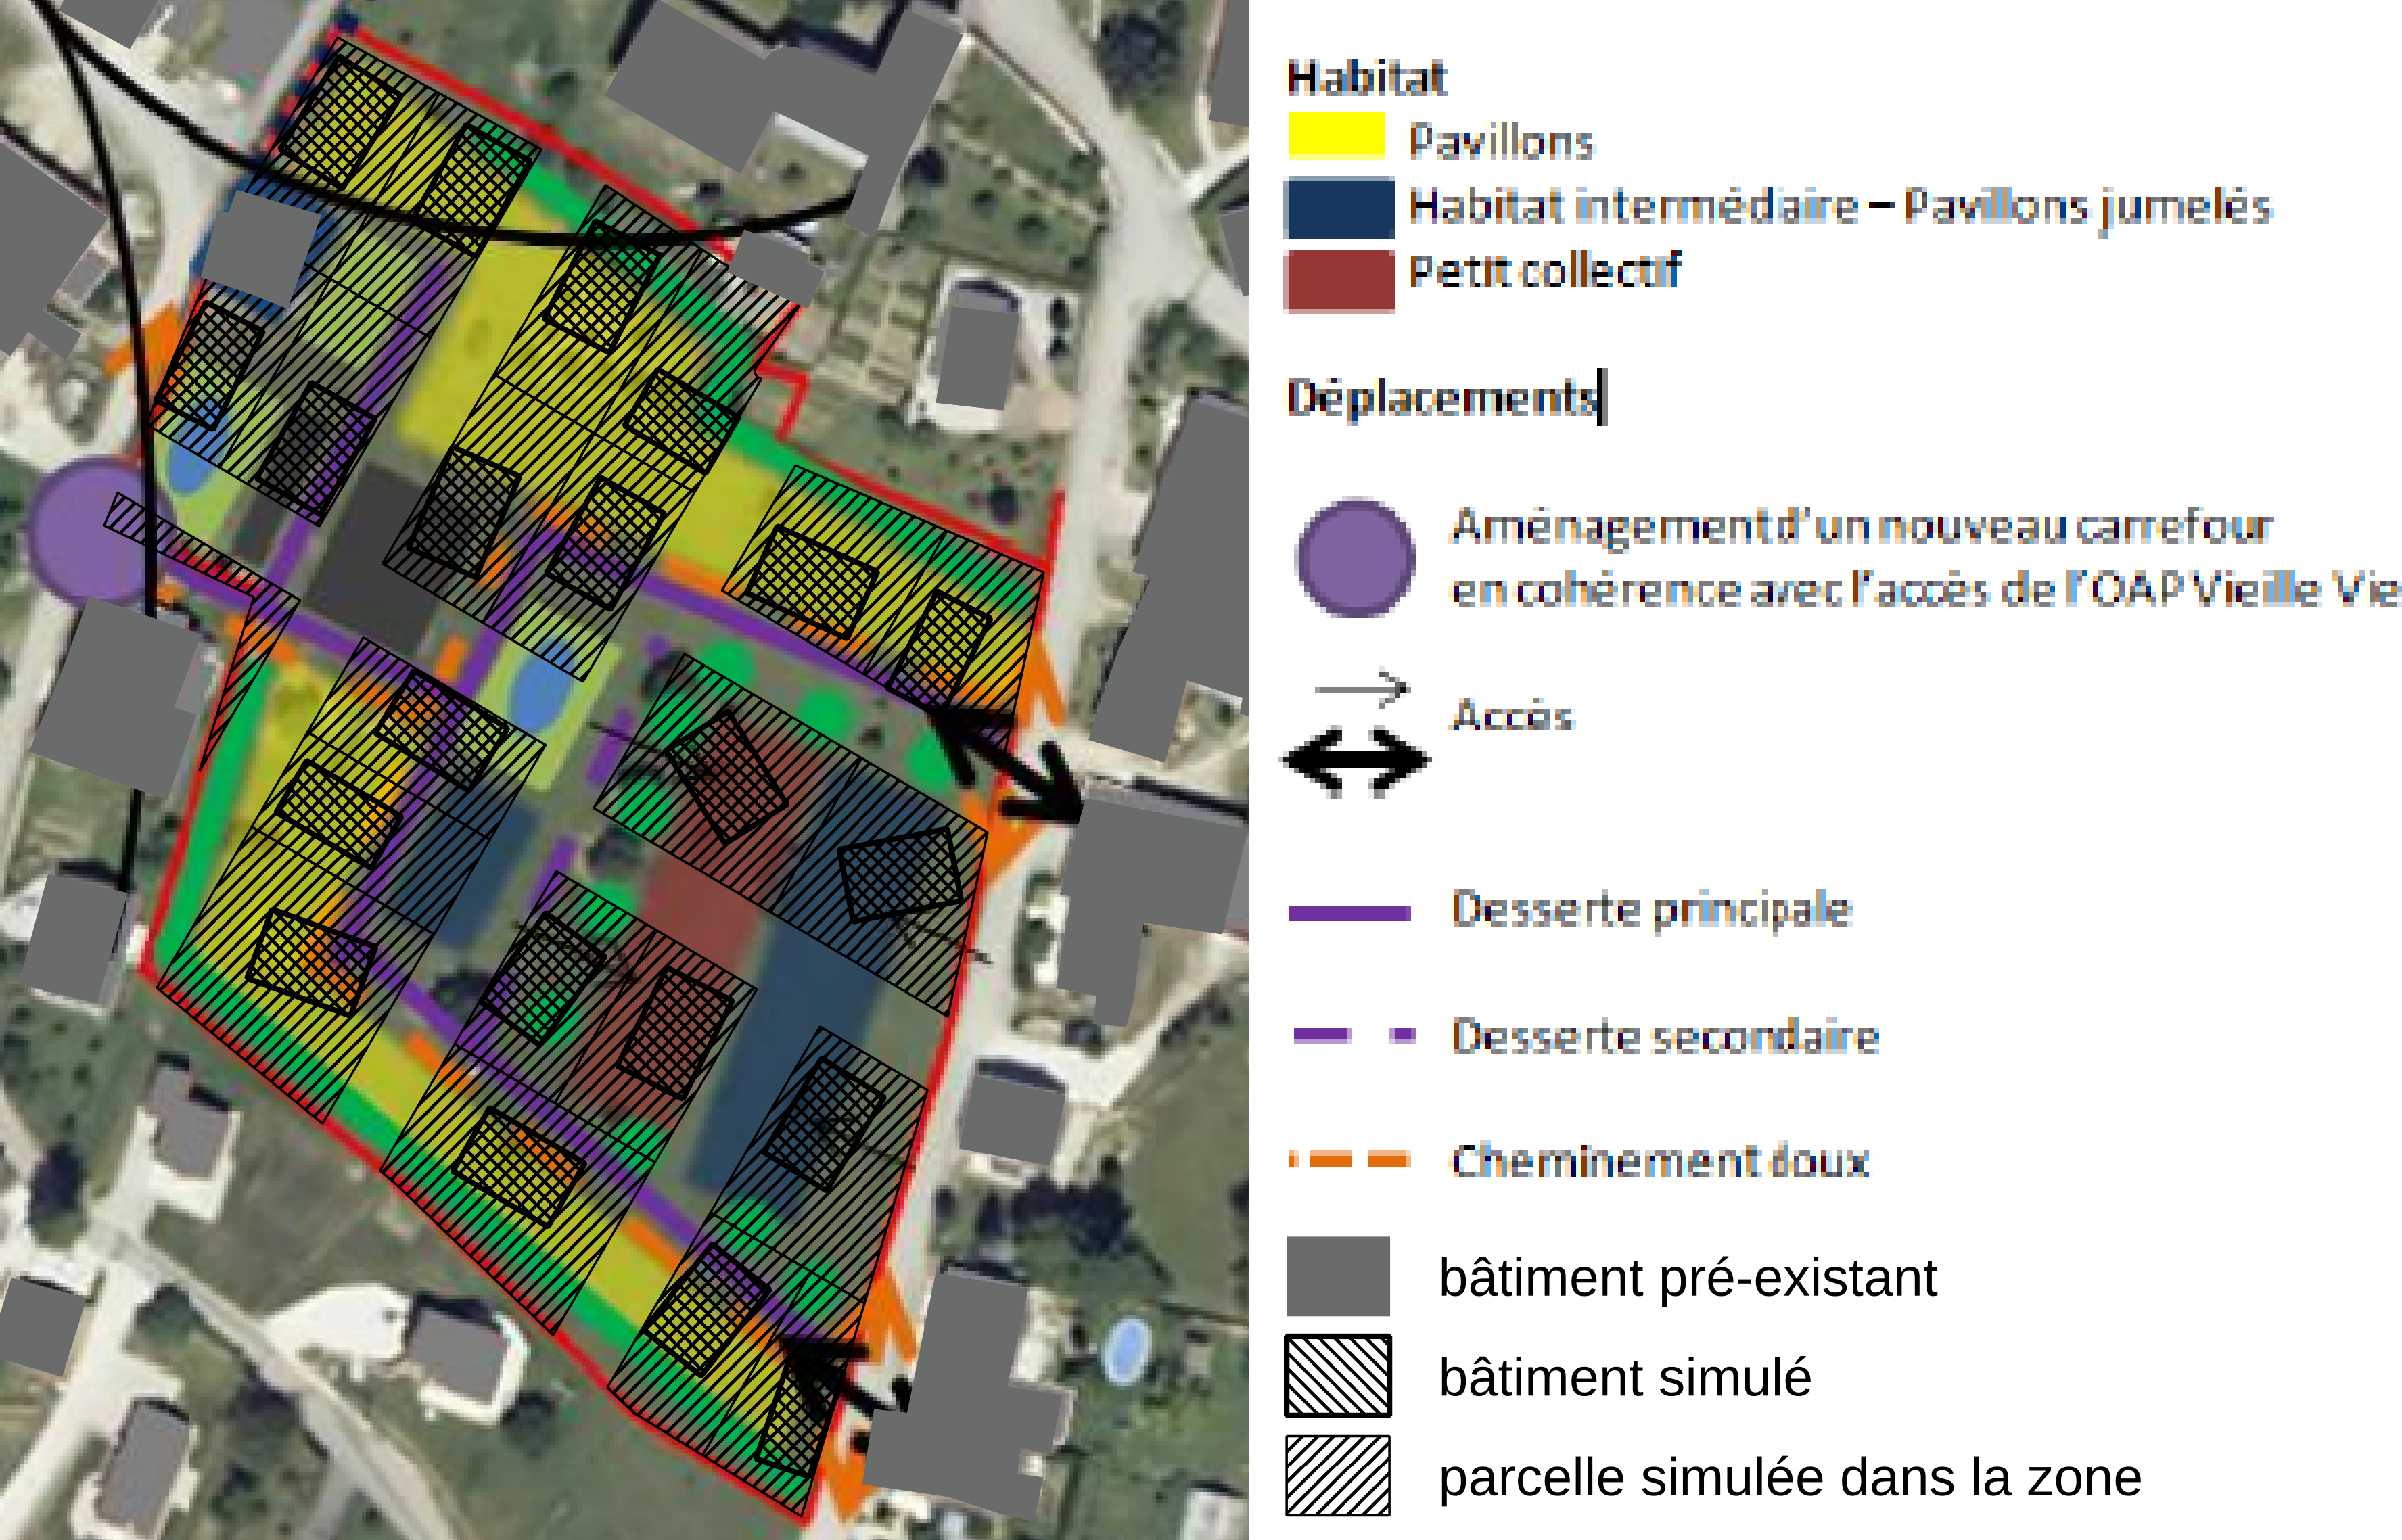
\includegraphics[width=9cm]{Images/OAPTour-de-Say2.png}
	\end{block}
\end{frame}

\section{Validation de SimPLU3D}

\begin{frame}{Validation de SimPLU3D}
	\begin{block}{Étude des paramètres de SimPLU3D}
		\begin{itemize}
			\item Étude du caractère aléatoire : très faible \textit{(Brasebin, 2014)}
			\item Étude de l'effet des paramètres scénaristiques~: \textit{(Chapron et al, 2017)}
		\end{itemize}
	\end{block}
	\uncover<2>{\begin{itemize}
		\item Pour chaque bâtiments~: estimations du nombre de logement et comparaison avec les attente pour le type de bâtiment
		\begin{itemize}
			\item Rétro-calcul si incompatibilité
		\end{itemize}
		\item \textbf{Validation thématique }de ces définitions de type de bâtiment 
	\end{itemize}}
\end{frame}




\section[Expérimentation]{Expérimentation d'ArtiScales sur l'agglomération du Grand Besançon}





\begin{frame}{ArtiScales : Expérimentation menée au cours de la thèse}
	\begin{block}
		\textbf{Objectifs de l'expérimentation}\\
		\begin{itemize}
			\item Évaluer le fonctionnement d'ArtiScales
%			\item Analyser les effets de la variabilité des simulation de MUP-City sur les résultats finaux 
			\item Vérification de son intérêt pour l'évaluation des documents de plannification et d'urbanisme
		\end{itemize}
	\end{block}
	\uncover<2->{
		\begin{block}{}
			Application à la Communauté d'Agglomération du Grand Besançon (CAGB)\\
				{\small Données d'entrées du modèle~:~2012\\}
			\vspace{0.1cm}
				\centering{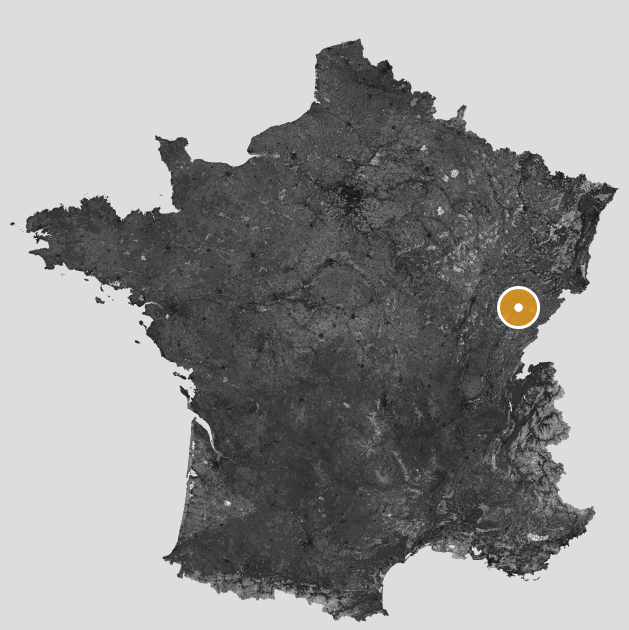
\includegraphics[width=3cm]{Images/france.png}}\\
		\end{block}
	}
\end{frame}

\begin{frame}{ArtiScales : Protocole des simulations}
	\begin{block}{Deux scénarios de développement résidentiel}
		\begin{itemize}
			\item Extension ciblée (développement résidentiel \textbf{contrasté}, \textbf{intense} et \textbf{extensif})
			\item Intensification (développement résidentiel \textbf{peu extensif} mais \textbf{uniforme} et \textbf{très intense})
		\end{itemize}
	\end{block}
	\begin{block}{Deux paramétrages de Parcel Manager et SimPLU3D}
	\begin{itemize}
		\item Forte augmentation de la densité
		\item Augmentation modérée de la densité
	\end{itemize}
\end{block}
\end{frame}

\begin{frame}{ArtiScales : Exécution du code informatique}
Pour ces quatre simulations~:
	\begin{itemize}
		\item temps \textbf{théorique} sur un ordinateur personnel~: \textbf{18 jours}
		\item temps \textbf{théorique} sur la grille de calcul européenne~: \textbf{6 heures}
		\item temps \textbf{constaté} sur la grille européenne~: \textbf{6 jours}
	\end{itemize}
\end{frame}

\section{Évaluation du fonctionnement d'ArtiScales}

\begin{frame}{ArtiScales : Densité nette de logements par $m^{2}$}
\pdfcomment{trois prochaines diapo soumises à un changement. Je vais également écrire mon texte pour être sur de ne pas aller trop dans le détail et dire tout ce qu'il faut}
\begin{table}[h]
	{\footnotesize \caption{Comparaison de la moyenne communale des densités nettes de logements par hectare entre le diagnostic du SCoT et les simulations d'ArtiScales}}	
	\tiny 
	\begin{center}
		\begin{tabular}{m{2.4cm}m{1.2cm}m{0.9cm}m{1cm}m{1cm}m{1cm}m{1cm}}
			\rowcolor[gray]{0.8}
			\multicolumn{3}{c}{Densité moyenne simulée pour le scénario~:}&\multicolumn{2}{c}{\textbf{étalement ciblé}} &\multicolumn{2}{c}{\textbf{intensification}}\\
			
			\rowcolor[gray]{0.9}
			Typologie de l'armature &
			Densité moyenne fixée par le SCoT &
			Densité moyenne observée&
			\cellcolor[gray]{0.8}paramétrage \textit{dense} & \cellcolor[gray]{0.8}paramétrage \textit{modérément dense}& \cellcolor[gray]{0.8}paramétrage \textit{dense} & \cellcolor[gray]{0.8}paramétrage \textit{modérément dense} \\ \hline
			
			Ville centre&50&60&45&56&49&57\\ \hline
			\rowcolor[gray]{0.9}Communes périphériques&23&21&22&16&23&17\\ \hline
			Communes relais &20&20&21&16&21&16\\ \hline
			\rowcolor[gray]{0.9}Communes équipées&15&12&16&14&17&15\\ \hline
			Halte ferroviaire&20&18&43&17&26&16 \\ \hline
			\rowcolor[gray]{0.9}Commune hors armature&13&13&18&15&19&16
			\\ \hline
		\end{tabular}
	\end{center}
\end{table}
\end{frame}

\begin{frame}{ArtiScales : Simulation de logements}
	\begin{table}[h]
		\caption{Comparaison de la création de logements mesurée par le SCoT avec les estimations des simulations d'ArtiScales}
		\label{Result:ConstLgt}
		\tiny
		\begin{center}
			\begin{tabular}{m{2.2cm}m{1.5cm}m{1.5cm}m{1.7cm}m{1.7cm}} 
				\rowcolor[gray]{.75}
				Typologie de l'armature&
				Objectif du SCoT sur 25 ans&
				Nombre de logements produits en 4 ans\footnote{d'après l'évaluation du SCoT sur la période 2012-2016}&
				Intensification - paramétrage \textit{dense} 
				& Étalement ciblé - paramétrage \textit{modérément dense} \\
				\hline
				Ville centre&18 200 \only<3>{(7 280)}&2 621&3 192&3 891\\\hline
				\rowcolor[gray]{0.9}Communes périphériques&3 500 \only<3>{(1 400)}&505&1 764&1 519\\\hline
				Communes relais &1 250 \only<3>{(500)}&147&489&331\\\hline
			 	\rowcolor[gray]{0.9} Communes équipées&600 \only<3>{(240)}&42&21&102\\\hline
				Halte ferroviaire&2 200 \only<3>{(880)}&328&948&1 207\\\hline
				\rowcolor[gray]{0.9}Commune hors armature&5 250 \only<3>{(2 100)}&1 055&2 718&4 729\\\hline %TODO ajouter les autres scenar
			\end{tabular}
		\end{center}
	\end{table}
	\only<2>{En 4 ans~: Production de logements en deçà des objectifs}
	\only<3>{De 2012 à 2016, on compte 60\% de \textit{renouvellement urbain}}
\end{frame}


\begin{frame}{ArtiScales : Comparaison avec les variantes}
A faire..
\\
Plus de comparaisons ciblée de scénarios
\\
Variantes serait un moyen de proposer des scénarios qui seraient ok? 
\\
Extrapolation du parcel manager
\end{frame}
\section{Utilisation thématique des résultats d'ArtiScales}

\begin{frame}{Compatibilité entre les documents}
	Incompatibilité entre les objectifs de création de logements et les documents d'urbanisme %(objectifs sur-dimensionnés ?)
	\\
	\only<1>{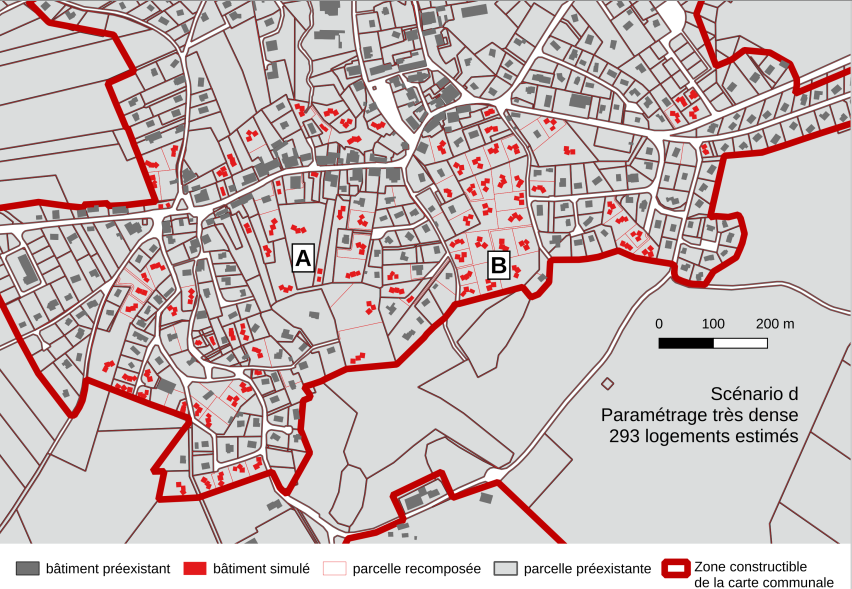
\includegraphics[width=8.7cm]{Images/nancray.png}}
	\only<2>{\textit{carte d'une commune qui ne peut pas atteindre les objectifs}}
	\only<3->{Possibilité de rétro-action~:
		\only<4>{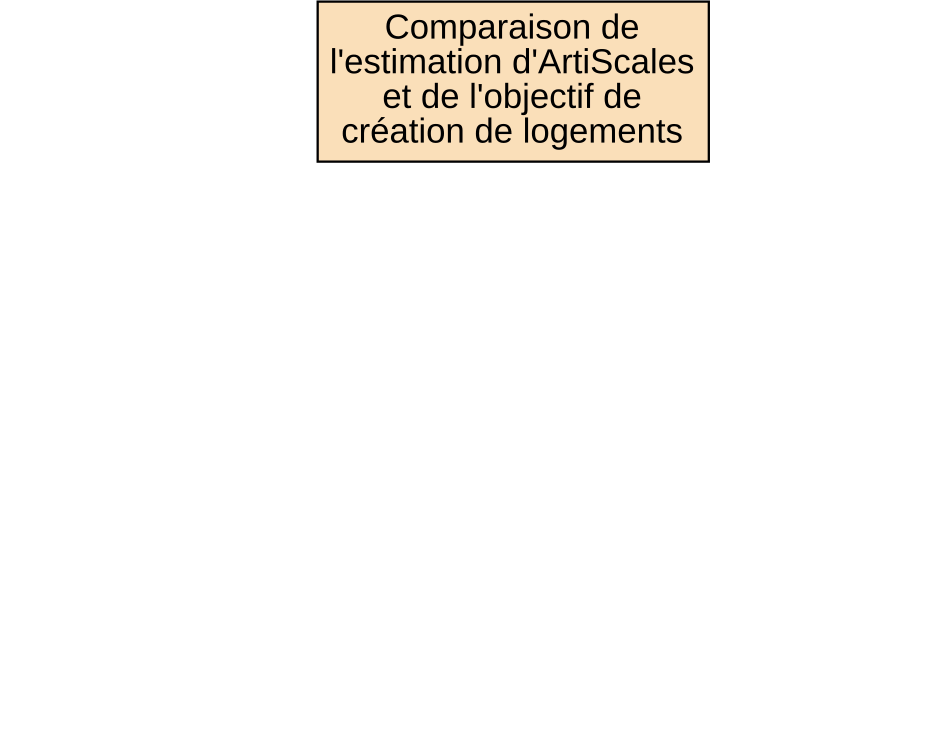
\includegraphics[width=7.7cm]{Images/schemCompatibleResult-prez0.png}}
		\only<5>{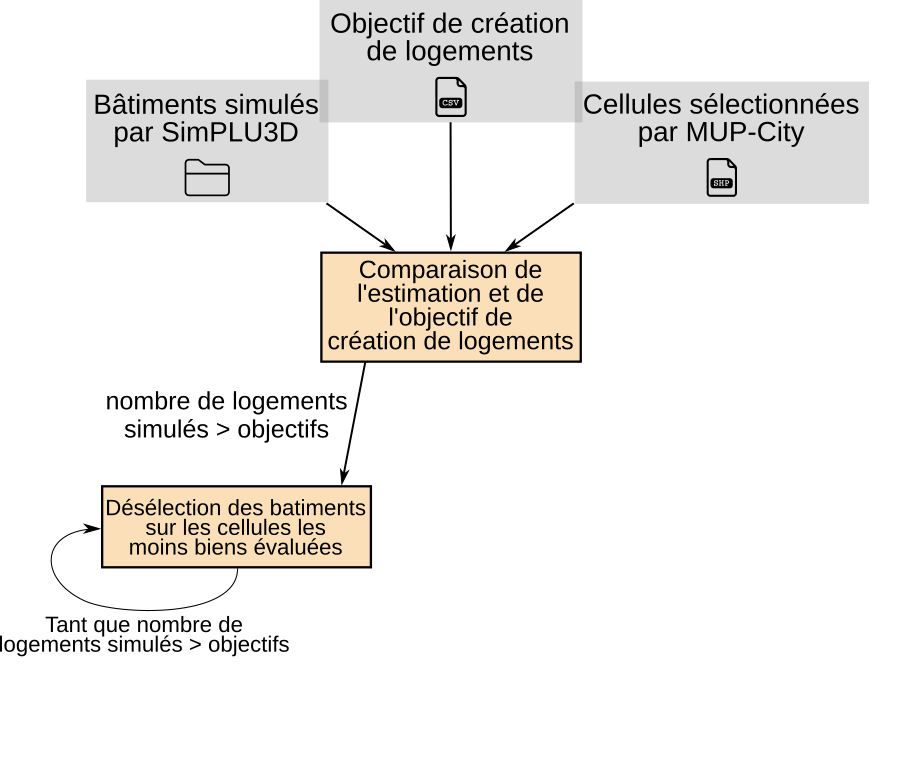
\includegraphics[width=7.7cm]{Images/schemCompatibleResult-prez1.png}}
		\only<6>{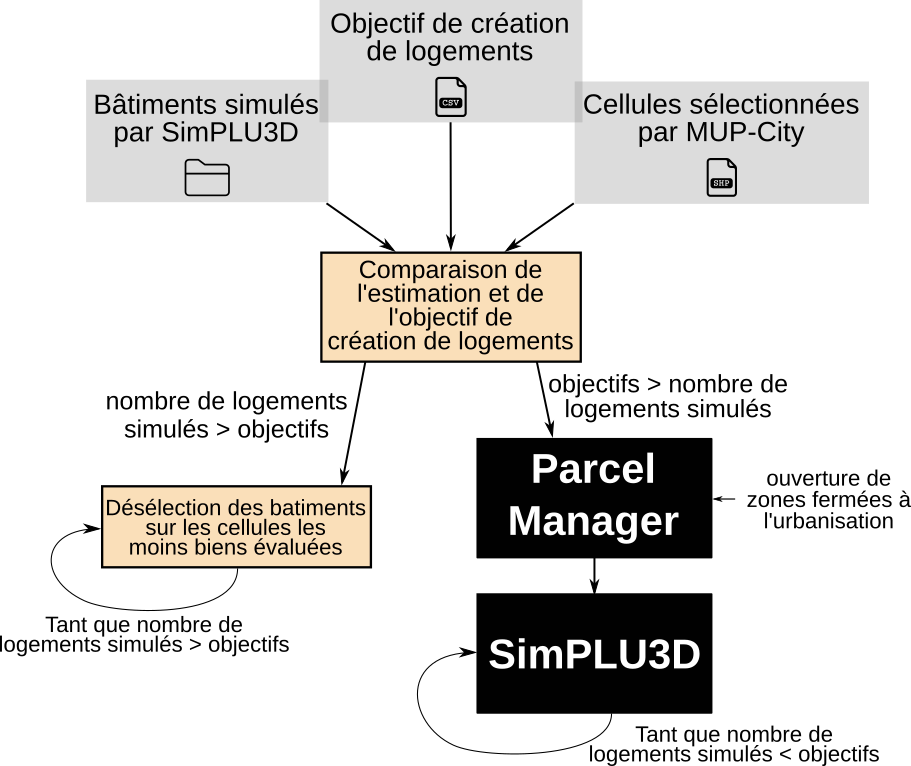
\includegraphics[width=7.7cm]{Images/schemCompatibleResult-prez2.png}}
	}
\end{frame}

\begin{frame}{Détecter la nécessité d'un zonage}
	Communes sans zonage pré-défini $\Longrightarrow$ ouverture de l'urbanisation dans les \textit{Parties Actuellement Urbanisée (PAU)}
	\\
	Les communes intéressantes à ubraniser soumises au RNU sont trop ouverte à l'urbanisation 
	\\
	\textbf{Necéssite d'un \textbf{zonage}}
	\\ %TODO refaire cette slide
	\textit{carte d'une telle commune}
\end{frame}

\begin{frame}{Possibilité de génération automatique de Cartes Communales}
Certaines communes n'ont pas de zonages et leur génération pourrait être automatisée~:
\begin{itemize}
	\item<2-> enveloppe des parcelles urbanisées
	\item<3-> ajout des parcelles les plus intéressantes à urbaniser, tout en 
	\begin{itemize}
			\item<4-> respectant les densités objectives et des objectifs de création de logements
			\item<5-> certifiant un certain non-étalement urbain
	\end{itemize} 
\end{itemize}
\end{frame}




\section{Conclusion et perspectives}




\begin{frame}{ArtiScales : Conclusions}
	\begin{block}{}
		\textbf{Simulateur hybride~:} couplage de \textbf{modèles génératifs} avec un \textbf{modèle stylisé} pour en faire un outil \textbf{opérationnel d'aide à la décision pour l'aménagement}
	\end{block}
	\begin{block}{}
		Résultats réalistes et plausibles au regard des évolutions du territoire
	\end{block}
	%	Pas de temporalité - peut être qu'une nouvelle itération devrait être faite tous les X ans ? % (cf rapport de 3 x pour chaque 4 ans) pour parvenir à remplir les objectifs ?
\end{frame}

\begin{frame}{Conclusion sur les modules utilisés par ArtiScales}
	\begin{block}{Utilisation de MUP-City :}
		\begin{itemize}
			\item variabilité intéressante pour proposer différentes configurations résidentielles
			\\
			\item plus adapté à générer une extension résidentielle
			\\
			\item possibilité de compléter ce module ? 			
		\end{itemize}
	\end{block}
	\begin{block}{Utilisation de SimPLU3D :}
		\begin{itemize}
			\item Optimisation de la simulation nécessaire
			\\
			\item Effet des paramètres techniques~: potentiellement important \textit{(soulevé par l'expérimentation de la thèse)}	\end{itemize}	
		\end{block}
\end{frame}
\begin{frame}{Apports de la thèse}
	\begin{itemize}
		\item Création d'un modèle de développement résidentiel complexe
		\item Analyse de la variabilité des modules composant ce modèle
		\item Utilisation de cette variabilité pour proposer différentes orientations d'aménagement
	\end{itemize}
\end{frame}

\begin{frame}{Perspectives d'utilisation d'ArtiScales dans l'aide à la décision territoriale}
	Rendre variable certaines restrictions afin de rendre compatibles entre eux les règlements.
	\\
	par exemple : 
	\begin{itemize}
		\item Zonage (expérimenté dans la thèse)
		\item Articles du PLU (hauteur, retraits)
		\item Objectifs de la planification (création de logements, densité...)
	\end{itemize}
	\uncover<2>{Mise en œuvre opérationnelle dans le cadre d'un contrat post-doctoral sur le PLU intercommunal de Besançon}
\end{frame}

\begin{frame}{Perspectives de recherche}
	\begin{block}{}
		Adapter SimPLU3D aux évolutions réglementaires suite aux lois ALUR et ELAN (plus de qualitatif (\textit{performantiel}) grâce à SimPLU3D)
	\end{block}
	\begin{block}{}
	\only<1>{Développer de nouveaux indicateurs pour évaluer les scénarios de développement résidentiel}
	\only<2>{\textbf{Développer de nouveaux indicateurs pour évaluer les scénarios de développement résidentiels}}
	\end{block}
	\begin{block}{}
	\only<1>{Automatiser l'analyse de variabilité pour permettre la génération de configurations spatiales intéressantes à urbaniser}
	\only<2>{\textbf{Automatiser l'analyse de variabilité pour permettre la génération de configurations spatiales intéressantes à urbaniser}}
\end{block}
\only<2>{
	\begin{block}{}
		Orienter la conception des documents d'aménagement vers des configurations résidentielles intéressantes
	\end{block}
}
\end{frame}



%\begin{frame}{D'un outil prospectif à un outil normatif}
%	Permettre de rédiger les documents d'urbanisme afin d'orienter le développement résidentiel
%	Nécessite le couplage avec d'autres approches ?
%\end{frame}
%\note{c'est peut être malin de ne pas proposer d'autre modèles pour faire la répartition et de laisser venir la question (quit à préparer une slide de réserve? Ou alors mettre ça dans les conclusions)
\begin{frame}[standout]
	\centering
	\begin{block}{}	
		\centering	
		Merci pour votre attention
	\end{block}
	\begin{block}{}
		\centering
		\textit{Everything we do is open source}\\
		\large
		\textbf{MUP-City}: \url{https://sourcesup.renater.fr/mupcity/} \\
		\textbf{SimPLU3D}: \url{https://github.com/IGNF/simplu3D}\\
		\textbf{ArtiScales :} \url{https://github.com/ArtiScales/}
	\end{block}
\end{frame}

\begin{frame}{Données nécessaire à l'exécution de MUP-City}
	\centering{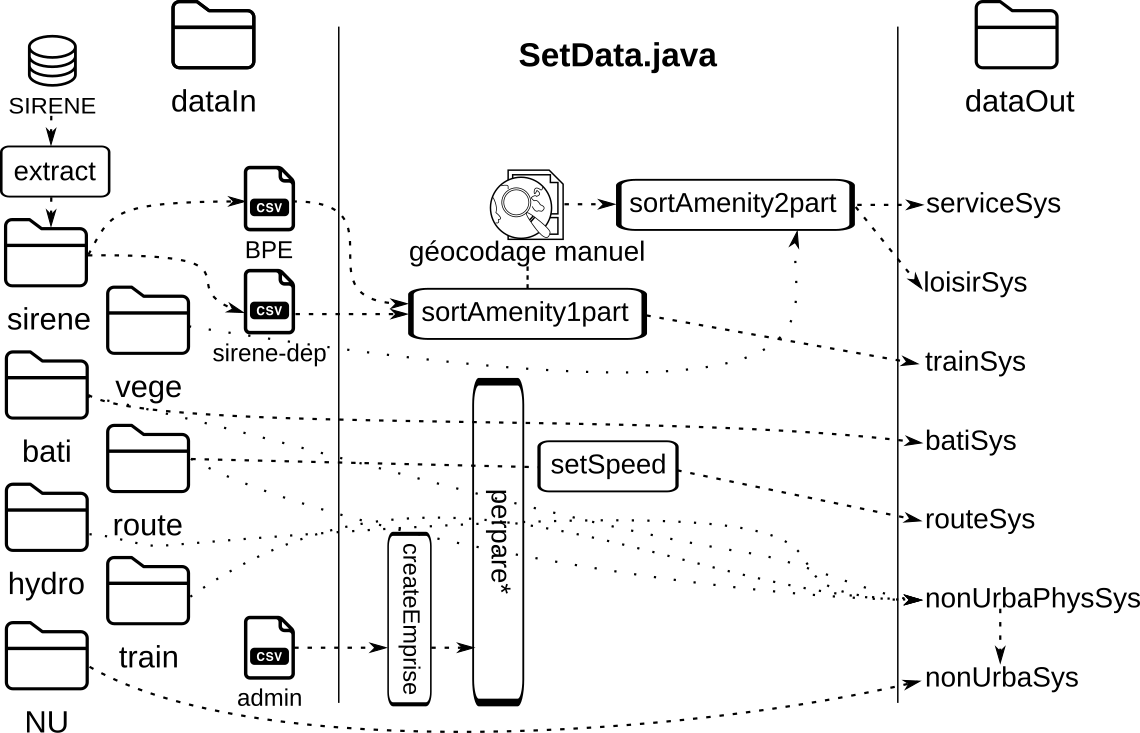
\includegraphics[width=10cm]{Images/schemaSetData.png}}
\end{frame}
\begin{frame}{Données nécessaire à l'exécution de SimPLU3D}
%		\centering{\includegraphics[width=8.5cm]{Images/simplu3DNbConfigs.png}}
%	\centering{\includegraphics[width=5cm]{Images/simplumodel.png}}
\end{frame}

\begin{frame}{Documents de planification régionale}
Le \textbf{Schéma de Cohérence Territoriale} (SCoT) \textbf{synchronise} les politiques territoriales régionales
\begin{itemize}
	\item Territorialise la construction de logements
	\item Fixe des contraintes morphologiques et de densité
\end{itemize}
\uncover<2->{Le \textbf{Programme Local de l’Habitat} (PLH) fixe la \textbf{politique du logement}
	\begin{itemize}
		\item Précise le nombre et le type de logements prévus par communes
		\item Programme de futures opérations
	\end{itemize}
	\uncover<3>{\textbf{Relation de compatibilité entre ces deux documents}}
}
\end{frame}

\begin{frame}{Documents de planification régionale - Exemple}
\includegraphics[width=11cm]{cartes/prevision-plh.png}
\end{frame}

\begin{frame}{Documents de planification locale - Les PLU}
Le \textbf{Plan Local de l’Urbanisme (PLU)} détaille et spatialise les contraintes de constructibilité au sein d’une commune
\begin{itemize}
\item a des \textbf{effets directs sur la constructibilité} mais ne planifie pas la construction 
\item \textbf{donne un cadre} pour la création de programmes de construction de logements \textit{(OAP, ZAC, ZAD)}
\item se compose en partie d'un \textbf{zonage} et d'un \textbf{règlement}
\end{itemize}
\end{frame}	

\begin{frame}{Application d'un PLU - Le zonage}
\begin{columns}[T]
\begin{column}[T]{7cm}
Zones générales et sous-zones particulières
\begin{itemize}
\item \alert{Naturelles} \textbf{(N)} \emph{non constructibles}
\item \alert{Agricoles} \textbf{(A)} \emph{non constructibles}
\item \alert{Urbanisées} \textbf{(U)}
\item \alert{À Urbaniser} \textbf{(AU)}
\end{itemize}
\end{column}
\begin{column}[T]{4cm}
\begin{textblock*}{6cm}(7.5cm,1.5cm)
\includegraphics[width=5cm]{cartes/plu-roche.png}
\end{textblock*}	
\end{column}
\end{columns}

\end{frame}

\begin{frame}{Rétro action pour la compatibilité en modifiant le zonage}
	
\end{frame}

\begin{frame}{Application d'un PLU - Le règlement}
\begin{columns}[T]
\begin{column}[T]{5cm}
Pour chaque sous-zone : 
\begin{itemize}
\item Articles 1, 2 : restrictions d’\textbf{usage du sol}
\item Articles 6, 7, 8 : \textbf{position des bâtiments} relativement aux autres bâtiments, aux limites de parcelles ou à la voirie
\item Article 10 : \textbf{hauteur maximale}
\item Article 11 : \textbf{aspect extérieur}
\end{itemize}
\end{column}
\begin{column}[T]{5.5cm}
\centering
\includegraphics[width=6cm]{Images/codesplu.png}
\\
\textit{Exemple de prescriptions graphiques (PLU de Strasbourg)}
\end{column}
\end{columns}
\end{frame}


\begin{frame}{ArtiScales : Sorties}
Pour l'ensemble de la zone d'étude~:
\begin{itemize}
	\footnotesize
	\item nombre total de bâtiments et de logements simulés, %différenciés en fonction de leur type et des \textit{secteurs} dans lesquels ils sont simulés.
	%	\item nombre et surface totale des parcelles sélectionnées, où des bâtiments ont pu être construits ou non, différenciés selon les \textit{secteurs} dans lesquelles elles se trouvent et selon les processus de recomposition parcellaires leur ayant été appliqués.
	\item emprise au sol totale et surface de plancher totale.
	\item densité (logements, surface au sol, surface de plancher) par surface de parcelles bâties.
\end{itemize}
Pour chaque commune~:
\begin{itemize}
	\item surface des parcelles où un bâtiment est simulé
	\item densité de l'ensemble de la commune après simulation.
	\item nombre de logements simulés et différenciés selon leurs types
	\item différentiel entre le nombre de logements créés et les objectifs de création de logements
	\item valeur moyenne (et écart type) de la densité de logements simulée et comparé aux objectifs
\end{itemize}
\end{frame}

\begin{frame}{Comparaison d'OAP et des résultats de simulation}
\only<1>{\textbf{Orientations d'Aménagement et de Programmation}~: Définition de l'organisation pour l'urbanisation de certaines zones. 
} 
\only<2>{
	\begin{table}
		\scriptsize
		\caption{Comparaison de la simulation utilisant le scénario \textbf{c} et un paramétrage induisant une \textit{forte densité} avec les objectifs de création de logements dans les OAP de Saône (25532)}
		\begin{tabular}{|m{3cm}ccccc|}
			Nom de la zone&Petite Saône&La Messarde&Au Cras&La Gilleroye \\ \hline
			Objectif de création \newline de logements &9&62&24&219 \\\hline
			Estimation d'ArtiScales&7&54&16&151 \\\hline
			Ressemblance des plans&non &oui&oui&non\\
		\end{tabular}
	\end{table}
}
\only<3>{
	\includegraphics[width=10cm]{Images/OAPTour-de-Say2.png}
	\\
	\tiny Illustration superposant l'OAP du \textit{Champ Sera} à La Tour De Say (25640) et les résultats de la simulation provenant du scénario \textbf{c} avec le paramétrage induisant une \textit{forte densité}
}
\end{frame}

\begin{frame}{Sélection parcellaire et consommation foncière}
\begin{table}
	\caption{Consommation foncière des différents scénarios}
	\scriptsize
	\begin{tabular}{|lcccc|}
		\hline 
		Scenario & \multicolumn{2}{c}{\textbf{Extension ciblée}} & \multicolumn{2}{c}{Intensification} \\ 
		Paramétrage densité & forte &modérée& forte&modérée\\
		\hline 
		Surface de parcelles urbanisée ($km^{2}$)& 6,267 &6,678&3,406& 3,859 \\	
		\hline 
		Surface de parcelles en zone urbanisée ($km^{2}$)& 3,867 &4,006&1,174& 1,368\\	
		\hline 
		Surface de parcelles en zone ouverte à l'urbanisation ($km^{2}$)&2,400&2,617&2,232&2,419\\ 
		\hline 
	\end{tabular} 
\end{table}
%	À titre de comparaison, 11,58 $km^{2}$ d’espaces artificialisés de 2001 à 2012
%	\\
\end{frame}

\subsection{Comparaison des variantes}

\begin{frame}{Présentation rapide des résultats des variantes}
\textit{pas sur d'en parler si ?}
\textit{min/max sur les quatre scénarios des tableaux et cartes pour situer ces différences}
\begin{block}{Neuf variantes de développement résidentiels}
	\vspace{0.1cm}
	Deux réplications de la modification des paramètres techniques~:
	\begin{itemize}
		\item graine aléatoire
		\item taille des cellules
		\item petits mouvements de la grille de décomposition
		\item grands mouvements de la grille de décomposition
	\end{itemize}
\end{block}
\end{frame}



\begin{frame}{Opportunités pour l'IGN}
%	\centering{\includegraphics[width=4cm]{Images/franceGPU.png}}\\
%	\FontPetit{\textit{Dépôt des PLU sur le GPU}}
\begin{itemize}
	\item Définition de données adaptées à la simulation des évolutions
	\item Proposition de service aux acteurs de la planification sur l'ensemble du territoire français
	\item Certification de la robustesse du processus de simulation relativement à la qualité des données
\end{itemize}
\end{frame}
\end{document}